% Created:  Sun 15 Jun 2014 04:15 pm
% @author Josh Wainwright
% File name : mainfile.tex

% \documentclass[a4paper,9pt,twoside,twocolumn]{extarticle}
\documentclass[a4paper,10pt,twoside]{article}
\usepackage[utf8]{inputenc}

%%% PAGE DIMENSIONS ------------------------------------------------------------
\usepackage[
	top=3.5cm,
	right=3.5cm,
	left=4cm,
	bottom=3cm]{geometry}
% \usepackage[top=3cm,
% 	bottom=2cm,
% 	left=1.5cm,
% 	right=1.5cm]{geometry}
\usepackage[parfill]{parskip}
\setlength{\columnsep}{1.5em}

%%% HEADERS & FOOTERS ----------------------------------------------------------
\usepackage{fancyhdr}
\pagestyle{fancy}
\fancyhf{}
\fancyhead[LE,RO]{\thepage}
\fancyhead[RE,LO]{Part \thepart}
\fancyfoot[CE,CO]{\thepage}
\fancyfoot[LE,RO]{}

%%% SECTION TITLE APPEARANCE ---------------------------------------------------
\usepackage{sectsty}
\allsectionsfont{\sffamily\mdseries\upshape}
\let\stdpart\part%
\renewcommand\part{\clearpage\stdpart}

%%% PACKAGES -------------------------------------------------------------------
\usepackage[hypcap=false,
	font=small,
	labelfont=bf,
	textfont=it]{caption}
\usepackage{subcaption}
\captionsetup{subrefformat=parens,width=8.8cm}

\usepackage[pdftex]{graphicx}
\usepackage{booktabs}
\usepackage{array}
\usepackage{longtable}
\usepackage{tabu} % \tabulinesep=1.2mm
\usepackage{multirow}
\usepackage{verbatim}
\usepackage{listings}
\usepackage[table]{xcolor}
\usepackage[binary-units]{siunitx}
\usepackage{amsmath}
\usepackage{enumitem}
\usepackage{url}
\usepackage{multirow,bigdelim}
\usepackage{nameref}

% \renewcommand{\labelenumii}{\theenumii}
% \renewcommand{\theenumii}{\theenumi.\arabic{enumii}.}
% \renewcommand{\labelenumiii}{\theenumiii}
% \renewcommand{\theenumiii}{\theenumii\arabic{enumiii}.}
% \usepackage[%
% 	activate={true,nocompatibility},
% 	final,
% 	tracking=true,
% 	kerning=true,
% 	spacing=true,
% 	factor=1100,
% 	stretch=10,
% 	shrink=10]{microtype}
% \microtypecontext{spacing=nonfrench}

%% CODE STYLING ----------------------------------------------------------------
\definecolor{grey}{HTML}{555753}
\definecolor{purple}{HTML}{75507b}
\definecolor{blue}{HTML}{3465a4}

\definecolor{dkgreen}{HTML}{4e9a06}
\definecolor{dkorange}{HTML}{8F5902}

\definecolor{lyellow}{HTML}{FCE94F}
\definecolor{lorange}{HTML}{FCAF3E}
\definecolor{lbrown}{HTML}{E9B96E}
\definecolor{lgreen}{HTML}{8AE234}
\definecolor{lblue}{HTML}{729FCF}
\definecolor{lpurple}{HTML}{AD7FA8}
\definecolor{lred}{HTML}{EF2929}
\definecolor{silver}{HTML}{D3D7CF}
\definecolor{lgrey}{HTML}{888A85}

\lstset{frame=tb,
	language=Java,
	aboveskip=3mm,
	belowskip=3mm,
	showstringspaces=false,
	captionpos=b,
	columns=flexible,
	basicstyle={\small\ttfamily},
	numbers=left,
	numbersep=-5pt,
	numberstyle=\tiny\color{grey},
	stepnumber=2,
	keywordstyle=\color{blue},
	commentstyle=\color{dkorange},
	stringstyle=\color{purple},
	breaklines=true,
	breakatwhitespace=true,
	tabsize=3,
	linewidth=8.8cm,
	morekeywords={function,each,in},
	escapeinside={(*@}{@*)},
	moredelim=[is][\color{dkgreen}]{|}{|}
}

%% BIBIOGRAPHY -----------------------------------------------------------------
\usepackage{cite}

%%% ToC (table of contents) APPEARANCE -----------------------------------------
\renewcommand{\contentsname}{Table of Contents}
% \setcounter{tocdepth}{2}

%%% PDF LINKS AND STYLE --------------------------------------------------------
\usepackage[bookmarks=true]{hyperref}
\hypersetup{%
	colorlinks=true, % false: boxed links; true: colored links
	linkcolor=black, % color of internal links (change box color with linkbordercolor)
	citecolor=black, % color of links to bibliography
	filecolor=black, % color of file links
	urlcolor=black   % color of external links
}
\hypersetup{pdftitle={Josh Wainwright MSc Project},
	pdfauthor={Josh Wainwright}}

\newcommand*\rfrac[2]{{}^{#1}\!/_{#2}}
\newcommand*{\fullref}[1]{\ref{#1}~\nameref{#1}}
%*******************************************************************************
%******************************** END HEADER ***********************************
%*******************************************************************************

\begin{document}

\graphicspath{{front/} {intro/} {grid/} {quadtree/} {clusters/} {plugin/}
	{analysis/} {improvements/} {appendix/} {build/}}

% Created:  Sun 15 Jun 2014 04:29 pm
% @author Josh Wainwright
% File name : titlepage.tex

\newgeometry{margin=1in}
\begin{titlepage}
	\begin{center}
		\vspace*{\fill}

		\centering
		
\includegraphics[scale=1.0]{Logo.pdf}
		\vfill

		\hrule
		{\LARGE\bf Medical Image Processing with Quadtrees\\[0.4cm]}
		\hrule

		\vfill
		\large
		School of Computer Science\\
		University of Birmingham

		\vfill
		Josh Wainwright
		\vfill

		\vfill
		\textit{Supervisor:} Iain Styles \\
		\vfill
		\textit{Date:} September 2014
		\vfill
		\vfill

	\end{center}
\end{titlepage}
\restoregeometry%

\newgeometry{onecolumn}
\thispagestyle{empty}
\pagenumbering{roman}

\textbf{Project Title:} Medical Image Processing with Quadtrees \\
\textbf{Author:} Josh Wainwright \\
\textbf{Supervisor:} Iain Styles \\
\textbf{Date:} September 2014 \\
\textbf{}
\vfill
\vfill

\subsubsection*{Declaration}

The material contained within this dissertation has not previously been
submitted for a degree at the University of Birmingham or any other university.
The research reported within this dissertation has been conducted by the author
unless indicated otherwise.\\

Signed \dotfill

\vfill
Submitted in conformance with the requirements of the post graduate degree of
MSc Computer Science at the School of Computer Science, University of
Birmingham (2013/2014).

\copyright~University of Birmingham 2013/2014
% Completed as part of a Post Graduate Masters Degree in Computer Science at the
% University of Birmingham (2013/2014).

\pagestyle{empty}

\newpage
\makebox[\linewidth][c]{%
	\begin{minipage}[c]{0.7\textwidth}
		\part*{Abstract}\label{prt:abstract}

		This project introduces the concept of data clustering and its uses in
		medical and biological image analysis and examines some existing
		techniques for extracting clustering information from such data sets. A
		new technique based on quadtree style data structures is discussed and
		an implementation tested and evaluated based on this technique. This
		method is found to perform well even under difficult conditions, such
		as noisy data, where others struggle, though has limitations in data
		set size, resource usage and taking advantage of parallel processing.

	\end{minipage}
}

\clearpage

\tableofcontents
\listoffigures
\addcontentsline{toc}{section}{List of Figures}
\listoftables
\addcontentsline{toc}{section}{List of Tables}
\lstlistoflistings%
\addcontentsline{toc}{section}{List of Code Listings}

\restoregeometry
\clearpage
\pagenumbering{arabic}
% \twocolumn
\pagestyle{fancy}


\setcounter{page}{1}
% Created:  Sun 15 Jun 2014 04:25 pm
% Modified: Thu 19 Jun 2014 05:22 PM
\part{Introduction}

\section{Medical Imaging}
\label{sec:section_name}

\section[Sub-Diffraction-Limit Imaging]{Sub-Diffraction-Limit\\ Imaging}
\label{sec:sub_diffraction_limit_imaging}

Imaging objects becomes more difficult as they get smaller because of the
wavelength of light. Once two objects are separated by a distance of an order
similar to that of the wavelength ($\lambda$) of the light used to view them,
it is no longer possible to resolve these two objects apart, instead all that
can be seen is a blur of the two objects together.

There have been several techniques developed for distinguishing objects apart
on smaller and smaller scales. Many of these involve using different
wavelengths of light.  For example, instead of being limited by visible light,
$\lambda \approx 5\times 10^{-7} \textrm{m}$, x-ray radiation ($\lambda \approx
10^{-10} \textrm{m}$) or even electrons ($\lambda \approx 10^{-11} \textrm{m}$)
can be used to resolve smaller scales in x-ray and electron microscopy
respectively. These, however, have the issue that, because the smaller
wavelengths imply higher energies, there is the danger of damaging the sample.
When imaging biological samples, this can be unreasonable.
%todo - unreasonable

\subsection{STORM}
\label{sub:storm}

Other techniques employ different methods of actually capturing the image, or
cleaver manipulation of the images that are produced, to get around the
limitations of the diffraction problem.

For example the STORM method\cite{rust2006sub} uses a technique where the
objects to be imaged are molecules of a fluorescent dye. The type of dye
molecule used allows the fluorescence to be switched on and off, allowing some
markers to be imaged separately to others, effectively increasing the distance
between points. Once an image is captured, the point spread function (PSF) of
the point is used to locate the single marker, the ``on'' markers are changed
and the image retaken.

% Created:  Sun 22 Jun 2014 11:25 AM
% @author Josh Wainwright
% File name : benchmarking.tex

\section{Benchmarking}
\label{sec:benchmarking}

Throughout the project, a set of files will be used to test the algorithms that
are developed; their correctness and effectiveness, speed and resource use.
Several of these files contain real data formated in the same way as would be
expected for data given to the plugin in general use, the others contain
simulated or uniform data for testing. The files that will be used are detailed
in Table~\ref{tab:benchmarking-files}.

\renewcommand{\arraystretch}{1.3}
\begin{table}[htbp]
\centering
\begin{tabular} {l r r}
	\toprule
	File Name & Size & Points \\
	\midrule
	\texttt{palm-1.txt} & \SI{12}{\mebi\byte} & 65572 \\
	\texttt{palm-2.txt} & \SI{6.4}{\mebi\byte} & 36672 \\
	\texttt{palm-3.txt} & \SI{5.8}{\mebi\byte} & 33342 \\
	\texttt{palm-3-small.txt} & \SI{176}{\kibi\byte} & 1000 \\
	\texttt{uniform.txt} & \SI{22}{\mebi\byte} & 2000000 \\
	\bottomrule
\end{tabular}

\caption[Sample data files used for testing and benchmarking.]{Files containing
	sample data are used for benchmarking throughout the project. A range of
	number of points per file, type of clustering expected for each file and
	the range of coordinates the points exist over is chosen to simulate
	different use cases.}\label{tab:benchmarking-files}
\end{table}

Note that \texttt{palm-3-small.txt} is a subset of \texttt{palm-3.txt} which
is used for simply checking correctness of algorithms. A summary of the
columns that are included in the files, used and unused fields, is included in
Appendix~\ref{app:data_file_structure} and a summary of the hardware that was
used when benchmarking the algorithms is shown in
Appendix~\ref{app:benchmarking_hardware}.

% Created:  Wed 13 Aug 2014 04:53 PM
% Author:   Josh Wainwright
% Filename: requirements.tex

\newgeometry{onecolumn}
\section{Requirements}
\label{sec:requirements}

% TODO Requirements intro
% TODO include explanation of MoSCoW

\subsection{Functional Requirements}
\label{sub:functional_requirements}

% TODO Functional Requirements

The plugin will allow the user to:

% \tabulinesep=1.2mm
% \newcounter{rowcount}
% \setcounter{rowcount}{-1}
% % TODO Don't have counter on header
% \begin{tabu}{@{\stepcounter{rowcount}\makebox[2em][r]{\therowcount.}\hspace*{\tabcolsep}}X c}
% 	\toprule
% 	Requirement & MoSCoW \\
% 	\midrule
% 	Select a data file to process.
% 	& M \\
% 	Select the appropriate column separator for the file.
% 	& C \\
% 	Select which coloumn the x- and y-coordinates appear in.
% 	& C \\
% 	Adjust parameters relating to the process of analysing the data file.
% 	& S \\
% 	Create an image of the points from the file using naitve ImageJ
% 	functionality.
% 	& S \\
% 	Perform a clustering algorithm on the data in the chosen file.
% 	& M \\
% 	Create an image of the clusters found using native ImageJ functionality.
% 	& M \\
% 	Generate perimeter information for each of the clusters found.
% 	& S \\
% 	Generate area information for each of the clusters found.
% 	& S \\
% 	Display a results table showing summary of information about each of the
% 	clusters found.
% 	& S \\
% 	Limit the clusters drawn to the image based on the size of the cluster.
% 	& C \\
% 	Limit the clusters included in the results table based on the size of the
% 	cluster.
% 	& C \\
% 	Export cluster information by selecing appropriate cluster from the results
% 	table.
% 	& W \\
% 	Export data points contained in cluster by selecing appropriate cluster
% 	from the results table.
% 	& W \\
% 	\bottomrule
% \end{tabu}

\begin{enumerate}
	\item Select data
		\begin{enumerate}
			\item Select a data file to process.
			\item Select the appropriate column separator for the file.
			\item Select which coloumn the x- and y-coordinates appear in.
			\item Adjust parameters relating to the process of analysing the
				data file.
		\end{enumerate}
	\item Create images
		\begin{enumerate}
			\item Create an image of the points from the selected file using
				naitve ImageJ functionality.
			\item Create an image of the clusters found using native ImageJ
				functionality.
		\end{enumerate}
	\item Perform a clustering algorithm on the data in the chosen file.
	\item Generate cluster information
		\begin{enumerate}
			\item Generate perimeter information for each of the clusters found.
			\item Generate area information for each of the clusters found.
			\item Display a results table showing summary of information about each of the clusters found.
			\item Limit the clusters drawn to the image based on the size of the cluster.
			\item Limit the clusters included in the results table based on the size of the cluster.
		\end{enumerate}
	\item Export data found by the algorithm.
		\begin{enumerate}
			\item Export cluster information by selecing appropriate cluster from the results table.
			\item Export data points contained in cluster by selecing appropriate cluster from the results table.
		\end{enumerate}
\end{enumerate}

\subsection{Non-Functional Requirements}
\label{sub:non_functional_requirements}

% TODO Non-Functional Requirements

The plugin will:

\begin{enumerate}
	\item Handle input data files of upto 3 million data points.
		% TODO test this
\end{enumerate}

\restoregeometry

% Created:  Mon 30 Jun 2014 05:32 PM
% Author:   Josh Wainwright
% Filename: rolling-ball.tex

\section{Existing Clustering Algorithms}
\label{sec:existing_clustering_algorithms}

A number of clustering algorithms already exist. Many of these are designed for
very specific purposes and so are not well suited for this application. Several
of these are described below.

\subsection{Rolling Ball Analysis}
\label{sub:rolling_ball_analysis}

The accessible surface area (ASA) algorithm, also known as the ``Rolling Ball
Method'', is a technique used in image processing for describing the outer
limit of a cluster of points. It is derived from biological molecules analysis
where it describes the surface area of a molecule that is accessible to a
liquid solvent.

The rolling ball method can be used to analyse a cluster of points by imagining
a solid ball or circle that sits against one of the outer-most points. From
here it is ``rolled'' around the cluster such that it is always touching at
least one point. Once the ball has reached the point it started at, the line
that the ball traced is reduced in size by the radius of the ball. This line
then represents the outer limit of the cluster.

The size of the ball must be chosen depending on the average separation of the
points within the cluster such that points classed as noise are not included
but all interesting points are.

\begin{figure}[tbhp]
	\centering
	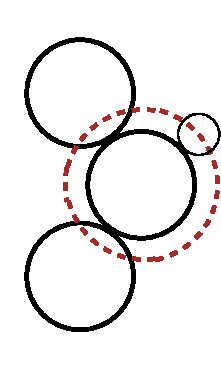
\includegraphics[width=4.2cm]{rolling-ball.pdf}

	\caption[Rolling ball method for cluster analysis.]{The rolling ball method
		for cluster detection provides a way of identifying clusters, as
		inspired by molecular biology. A very simple implementation can be fast
		but is not particularly successful at finding clusters unless the data
		points are very dense and there is no noise.}\label{fig:rolling-ball}
\end{figure}

A simple approximation of this technique can be achieved by using the same
dilating and eroding processes that are described later in
Section~\ref{sec:simple_grid_method}.

\subsection{Shared Nearest Neighbours}
\label{sub:shared_nearest_neighbours}

Shared nearest neighbour (SNN) clustering algorithms have been used to overcome
some of the problems encountered with more traditional clustering methods when
working in higher dimensions. In these cases, simple Euclidean geometry becomes
unable to cope with the computation and so is replaced with other coordinate
systems. For simple clustering in two dimensions, however, Euclidean geometry
is sufficient and is far easier and more efficient to implement.

SNN based clustering algorithms analyse each of the points in a set, one at a
time, selecting those points that lie close to the current one based on certain
thresholds. As the algorithm progresses, these thresholds are altered and the
points considered so far are re-examined to maximise the ``similarity'' of the
points in any one cluster.

Implementations of SNN based algorithms, such as~\cite{jarvis1973clustering}
and~\cite{ertoz2002new} use similarity matrices, where the set of points is
reduced to a graph with the data points at nodes and the edges between them
representing the similarities between the points. This matrix is then
simplified to leave a considerably sparser graph, keeping only the edges with
the highest similarity. From this matrix, points can be identified as noise and
rejected, and the networks that show close similarities are designated as
clusters.

This method is very good at being adaptable to complex situations: arbitrary
dimension, clusters with complicated shapes, high noise levels, etc. However,
the complexity in implementation and computation makes it unsuitable for small
scale clustering such as the application discussed for this project. It also
suffers from performance issues when the number of points to analyse becomes
large as it has approximately $O(n^2)$ time complexity.

\subsection{Gravity Based Clustering}
\label{sub:gravity_based_clustering}

A number of clustering algorithms~\cite{zhong2010novel} have been developed
that treat data points as physical objects under the influence of gravitational
effects.  These algorithms effectively model the points with these properties,
allow them the move with some defined restrictions, and then examine the
products that are produced.

The GRAVIclust algorithm~\cite{indulska2002gravity} works in two phases, first
identifying $n$ locations of interest based on the distances to neighbouring
points, similar to the SNN algorithms above, and secondly applying an
optimisation phase where each of these locations is further examined with the
gravity effects of other points applied.

Unfortunately, these algorithms require certain information about the data set
before clustering can be performed. First, a matrix of the distances between
every pair of points must be calculated. This make working with large data sets
prohibitive. Second, the number of clusters to identify is required. This means
that an algorithm to search for arbitrary numbers of clusters is not possible.

% Created:  Tue 01 Jul 2014 03:19 PM
% Modified: Tue 01 Jul 2014 03:19 PM

\part{Data Structures}
\label{prt:data_structures}

%TODO
The way in which the data is represented in memory


% Created:  Mon 23 Jun 2014 13:15 PM
% @author Josh Wainwright
% File name : grid.tex

\section{Uniform Discrete Cell Method}
\label{sec:simple_grid_method}

The simplest method for analysing the distribution of points is to use a
uniform, discrete grid of cells and place the points into these cells one at a
time. Once all points have been added, the number of points that are contained
in each cell can be treated as a grey scale brightness value with lighter
pixels representing cells with more points and black cells having no points.
This gives a simple pixel image, with brightness as a function of density of
the points, in the \texttt{pnm} image format\cite{murray1996encyclopedia}. A
thresholding filter can then be applied to remove the points that are isolated
by removing the darker pixels and leave the denser areas corresponding to
clusters.

Though the resolution of this method can be easily changed by altering the size
of the cells in the grid, it performs badly when presented with data that is
even slightly noisy. If the clusters themselves have a density that is not
significantly above the background noise level, the thresholding step is prone
to either exclude much of the interesting data, or to increase the size of the
clusters by including too much noise. These two effects can be seen clearly in
Figure~\ref{fig:grid-noise}, where \texttt{palm-1.txt} is used with a cell size
of 200. The range of the data is from 0 to \num{41000} for both the $x$ and the
$y$ axes, thus the images are $\left(\rfrac{41000}{200} = \right)$ 205 by 205
pixels. This data took \SI{495}{\milli\second} to generate.

\begin{figure}[tbh]
	\centering
	\begin{subfigure}[b]{4.2cm}
		\frame{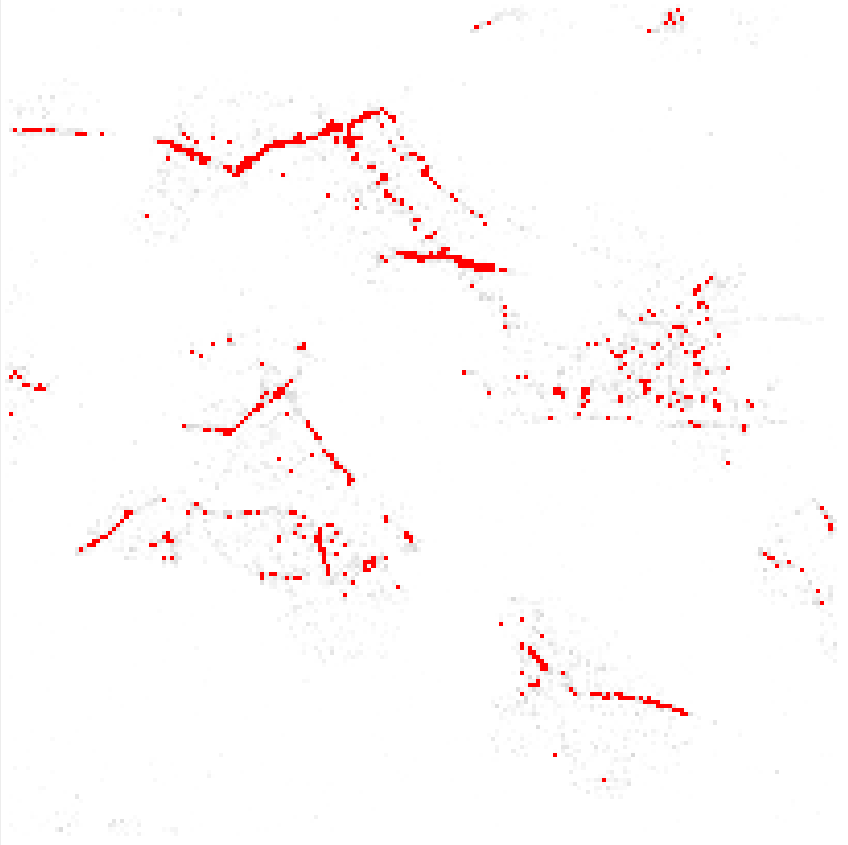
\includegraphics[width=\textwidth]{grid-noise-low.png}}
		\caption{}\label{fig:grid-noise-low.png}
	\end{subfigure}%
	\quad
	\begin{subfigure}[b]{4.2cm}
		\frame{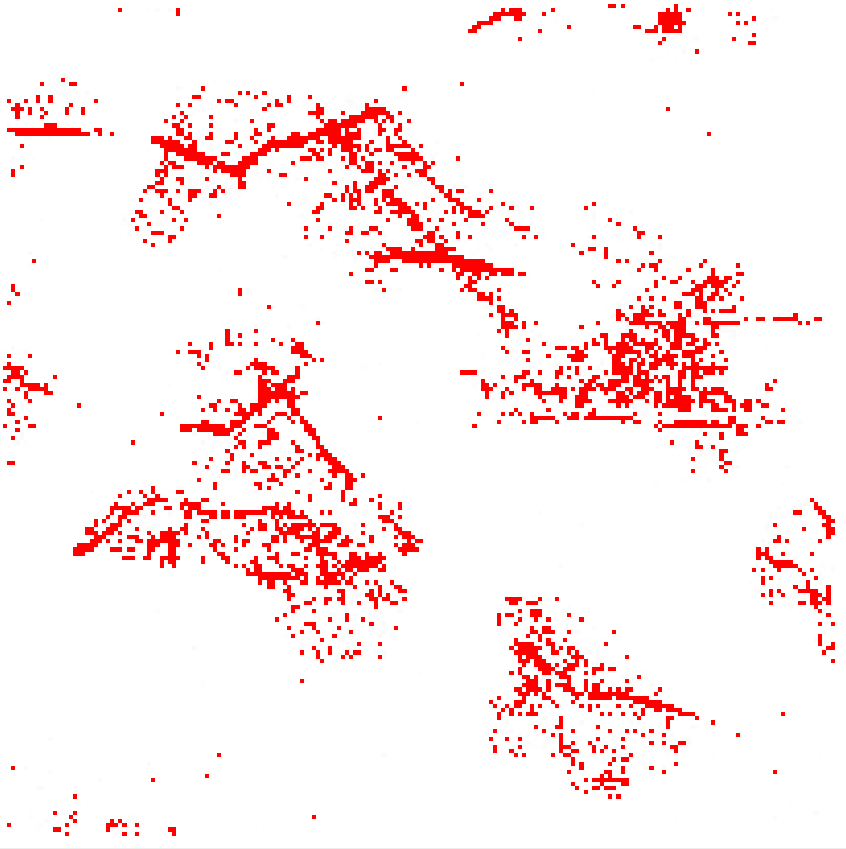
\includegraphics[width=\textwidth]{grid-noise-high.png}}
		\caption{}\label{fig:grid-noise-high.png}
	\end{subfigure}

	\caption[Effect of threshold value on clusters identified.]{Setting a low
		threshold, \subref{fig:grid-noise-low.png}, means that many of the
		points in the clusters are lost. Setting it higher,
		\subref{fig:grid-noise-high.png}, includes too many of the points
		deemed to be noise. Red pixels are ones that would be kept by the
		thresholding process, black would be removed.}\label{fig:grid-noise}
\end{figure}

There are a few steps that can be taken to improve the approach of this simple
grid when handling outlying points caused by noise:

\begin{enumerate}

	\item First the algorithm is modified to include a thresholding step before
		writing the pixel image data to a file. This means that the pixels can
		be adjusted with greater accuracy and any arbitrary level can be chosen
		to threshold at.

	\item Next, once the image has been generated, the number of points that
		contributed to each pixel is no longer of interest and so the image can
		be converted to a binary image. This is an image with just two possible
		values, the first represents white space, where there are no points,
		the seconds is black where there were points and so is of interest.

	\item Once a binary image has been generated, dilate and erode filters can
		be applied to remove remaining outliers and to try to close the gaps in
		the structures that have been identified so that they are more solid.

\end{enumerate}

\begin{figure}[tbh]
	\centering
	\frame{
\includegraphics[width=7cm]{grid-threshold-close.png}}

	\caption[Closing algorithm to identify clusters.]{Using dilating and
		eroding algorithms can help to emphasise the structure in the
		data and, at the same time, remove the isolated points representing
		noise.}\label{fig:grid-threshold-close}
\end{figure}

These steps lead to significantly better isolation of the interesting parts of
the image, as can be seen in Figure~\ref{fig:grid-threshold-close}, however,
much of the detail of the structure is lost in this process.

% Created:  Fri 27 Jun 2014 11:24 AM
% Author:   Josh Wainwright
% Filename: quadtree.tex

\section{Quadtrees}
\label{sec:quadtrees}

Since the simple grid method described in Section~\ref{sec:simple_grid_method}
performs slowly and does not offer good cluster analysis, a different approach
is needed. The chosen method is to use a quadtree data structure.

Quadtrees are a type of recursive abstract data type in the form of a tree
where every node has exactly zero or four children. A node with zero children
is a leaf and contains some information, value or quantity. A node with four
children is not a leaf and cannot hold information.

Quadtrees are often used in image processing since the four children of the
root node can naturally represent the four quadrants of the image; upper left,
upper right, lower left and lower right. Since each of these children is also a
quadtree, the image can be subdivided to any arbitrary depth. From this point,
information about the image can be ``seen'' more easily by the computer and
statistics calculated.

\subsection{Quadtree Definitions}
\label{sub:quadtree_definitions}

It is useful to define a few terms that shall be used in the context of
quadtrees. Many of these are identical to the definitions more commonly applied
to binary trees.

\begin{description}
	\item[Node] (Cell) A leaf in the tree which holds a number of points.
	\item[Root] The node at the topmost position in the tree.
	\item[Child] One of the four nodes that are beneath a given node for which
		there is a direct path of length 1 between this node and it.
	\item[Height] The length of the longest path from the root node to one of
		the leaf nodes.
	\item[Depth] The length of the path from a given node up to the root.
	\item[Completeness] A quadtree is `complete' when each of the root node's
		four children have the same height. In this case, the number of leaves
		in the tree is a maximum.
	\item[Quadtree Code] (Code) The unique binary number assigned to a node by
		adding its position with respect to its siblings to the code of its
		parent.
\end{description}

\subsection{Code Orderings}
\label{sub:code_orderings}

In order to identify a node uniquely in the tree, each node is given a code
that is built up from it's parent code plus some value that identifies it
among it's siblings. The root node is usually chosen to have an empty code so
that the first four children are given the first level codes.

The choice of what order to label the children is important if the order
in which the nodes are placed is important. For spatial indexing, for example,
each node represents a quadrant in two dimensional space, so being able to
traverse the children in a sensible and predictable way is essential.

\begin{figure}[tbhp]
	\centering
	\begin{subfigure}[b]{3.5cm}
		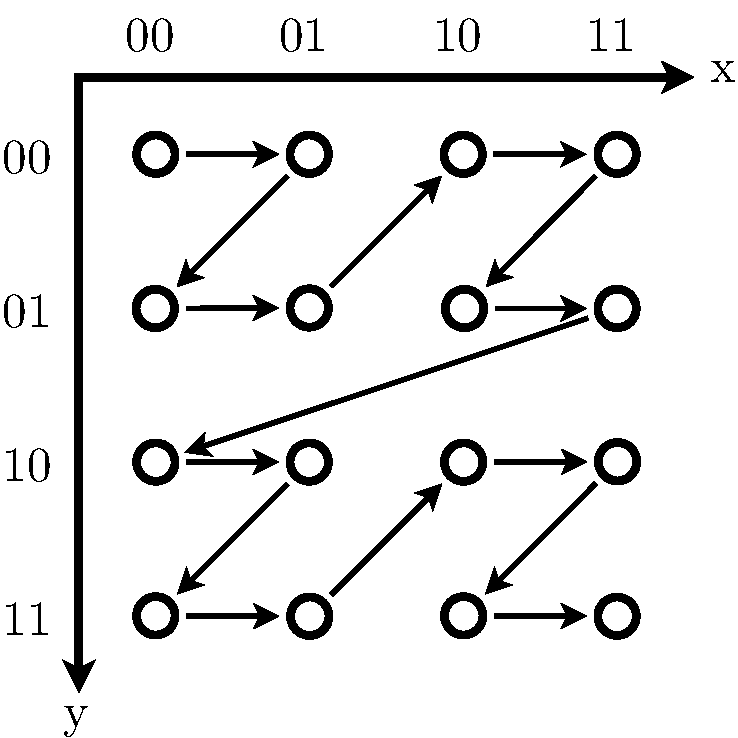
\includegraphics[width=\textwidth]{traverse-z-order.pdf}
		\caption{}\label{fig:traverse-z-order.pdf}
	\end{subfigure}%
	\quad
	\begin{subfigure}[b]{3.5cm}
		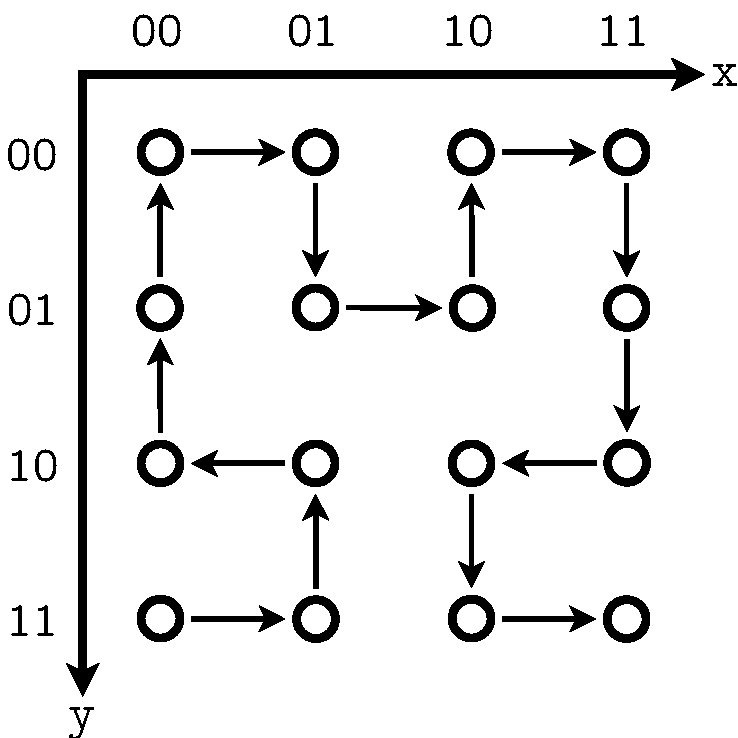
\includegraphics[width=\textwidth]{traverse-hilbert-order.pdf}
		\caption{}\label{fig:traverse-hilbert-order.pdf}
	\end{subfigure}
	\\[0.2cm]
	\begin{subfigure}[b]{3.5cm}
		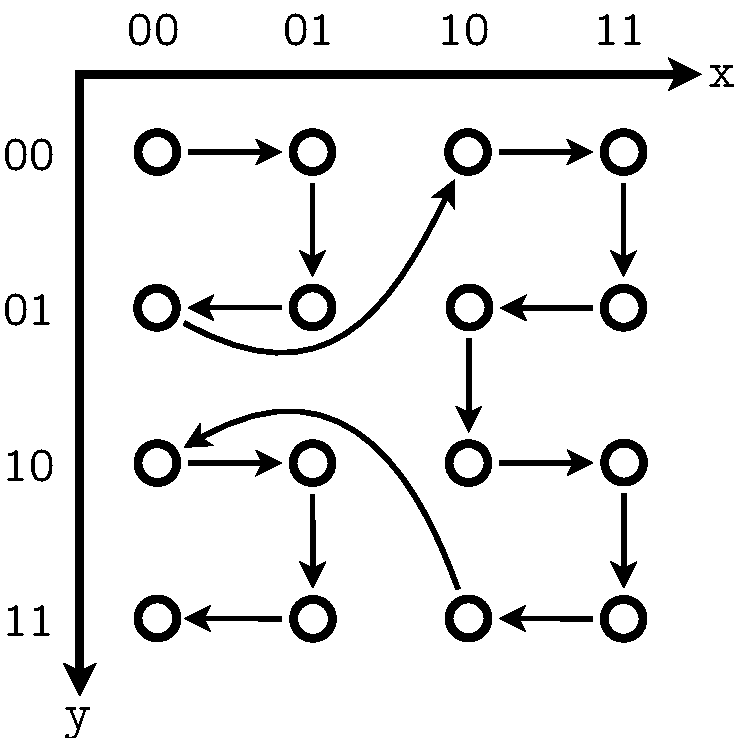
\includegraphics[width=\textwidth]{traverse-gray-order.pdf}
		\caption{}\label{fig:traverse-gray-order.pdf}
	\end{subfigure}%
	\quad
	\begin{subfigure}[b]{3.5cm}
		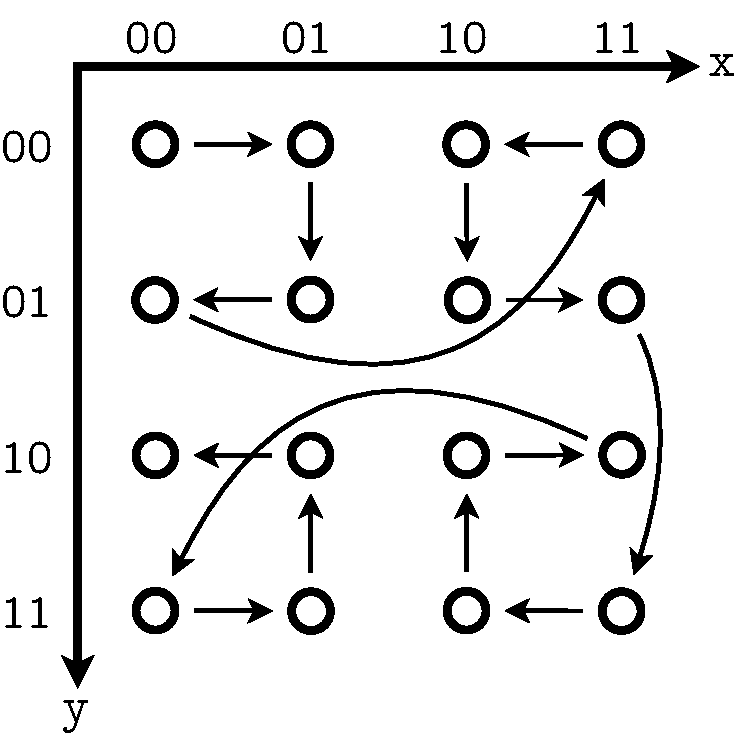
\includegraphics[width=\textwidth]{traverse-modgray-order.pdf}
		\caption{}\label{fig:traverse-modgray-order.pdf}
	\end{subfigure}

	\caption[A selection of possible tree traversal orderings]{A selection of
		possible tree traversal orderings. Each of theses is, more formally, a
		space filling curve which is a direct, unique mapping from a 2D grid to
		a 1D array. \subref{fig:traverse-z-order.pdf} shows Z-order,
		\subref{fig:traverse-hilbert-order.pdf} shows Hilbert order,
		\subref{fig:traverse-gray-order.pdf} shows Gray code order and
		\subref{fig:traverse-modgray-order.pdf} shows the modified Gray code
		order developed for this project.}\label{fig:order_traversals}
\end{figure}

\subsubsection[Morton Order]{Morton Order (Z-Order)}
\label{ssub:morton_code_z_order_}

Perhaps the most natural order to give to the values in a spatial quadtree is
to number them from 1 to 4, left to right, top to bottom. This can be made
more appropriate for a computer to use by numbering from 0 to 3. This is
called Morton Order\cite{mortoncomputer} or Z-order because of the resulting
path that would be followed by traversing the nodes in order,
Figure~\ref{fig:traverse-z-order.pdf}. This has several useful features.

\begin{enumerate}
	\item First, the numbers can be converted to base 2:
	\begin{itemize}
		\item 0 becomes 00
		\item 1 becomes 01
		\item 2 becomes 10 and
		\item 3 becomes 11.
	\end{itemize}

	\item This has advantages since binary is very efficient for computers to
	work with and allows certain tricks to be employed (see Morton order
	coordinates).

	\item Also, this numbering system is easily extendible to any depth of
	tree that can be imagined.

	\begin{enumerate}
		\item The root, as mentioned before, is given no value,
		\item each of the children are numbered {00} through 11.

		\item the children of these children are numbered 00 to 11 with the
		parent as a prefix. So the children of node 00 are 0000, 0001, 0010
		and 0011. Likewise, the children of 11 are 1100, 1101, 1110 and 1111.

		\item The children are always numbered in the same order. If starting
		at the top and going top to bottom and left to right, this is
		maintained for all children.
	\end{enumerate}
\end{enumerate}

This method of numbering is simple and so acceptable for the standard uses of
quadtrees, but it was found to be difficult to work with in a spatial context
when information about neighbouring cells is needed. The steps required to
calculate the neighbours of any given cell are reasonably complex and so would
add computational and time complexity to calculations performed on the tree.

\subsubsection*{Morton Order Coordinates}
\label{ssub:morton_order_coordinates}

Another useful feature of the Morton ordering is the simple conversion from
quadtree code to Cartesian coordinate notation. The steps to convert to
coordinate form are:

\begin{enumerate}
	\item Ensure the code is in binary format with two bits for each level of
		the tree.
	\item \emph{De-interleave} the bits of the code (starting with the first
		being given to the $y$-axis, assign bits to the $y$ and $x$ axes
		building up a binary value for each).
	\item Convert the resulting two binary value to decimal to give a standard
		decimal $(x,y)$ coordinate.
\end{enumerate}

\begin{figure}[tbhp]
	\centering
	\includegraphics[width=0.8\linewidth]{deinterleave.pdf}

	% TODO caption
	\caption{Deinterleave}\label{fig:deinterleave}
\end{figure}

This method means that it is very easy to calculate an arbitrary number of
nodes in any direction by simply converting the code for a node to coordinates,
adding or subtracting the number of positions to move in the $x$ and $y$
directions and then converting back to quadtree code representation by
following the algorithm above in the reverse order.

Of course, this method has no knowledge of the structure of the quadtree being
used and so only provides the code of the node that would occupy the space at
the given coordinate. That node might not exist---the tree might not extend
deep enough, so the node in that position is larger than expected; or the tree
might be deeper at that location meaning the node is smaller. In these cases,
there are a number of options as to how to find the correct node for the code:

\begin{itemize}
	\item The code can be shortened and/or lengthened and the resulting adapted
		code checked to see if it is in the tree. This trial and error method
		can be fastest when there is a limit on the depth range allowed when
		searching (see Section~\ref{sub:algorithm_description}).
	\item The tree can be traversed to find the nearest node to the expected
		code reference.
\end{itemize}

\subsubsection{Hilbert Order}
\label{ssub:hilbert_order}

One of the reasons the Z-order above becomes difficult to work with is that
the resulting path from traversing the nodes in-order has to make large jumps
and so cells which are numbered next to each other may, in fact, not be near
each other in the image.

A number of routes exist that avoid this jumping around the image. These are
based on space filling curves which have the property of being a simple
recursive pattern that visits every point in a 2D space exactly once. These
curves were first discovered in the early 1900's and described mathematically
by D. Hilbert\cite{hilbert1970stetige}. One of the curves that Hilbert found,
the Hilbert Curve, is particularly useful since it can be represented in the
simplest level in a two by two square which is then recursively repeated for
each quadrant of that first square---exactly as the quadtree does.

The path that the traversal of points follows becomes fairly complicated,
Figure~\ref{fig:traverse-hilbert-order.pdf}. This means, again, that the
calculation of neighbours becomes difficult.

\subsubsection{Gray Codes}
\label{ssub:gray_codes}

The Gray Code\cite{gray1953pulse}, developed by Frank Gray in 1953, was
originally designed to reduce the error rate produced by mechanical
electronics. The code is a variation on binary where each step when counting
up changes only a single bit at a time. This meant that electromechanical
apparatus was less likely to make a mistake or generate errors since the
actions required to count from one to two required only a single bit change,
rather than two, as would be required for binary counting. When using just two
bits, i.e., counting from zero to three, the steps are very similar to binary,
(00, 01, 11, 10).

The path that this follows is shown in
Figure~\ref{fig:traverse-gray-order.pdf}. This does not seem to provide any
benefits since there is now more jumping around the image space than with
Z-order and the neighbours are just as difficult to calculate as for Hilbert
Order. However, by using a different arrangement of the sub-trees, as the
Hilbert curve does, the leaf nodes group themselves in a very ordered
fashion. When arranged as in Figure~\ref{fig:traverse-modgray-order.pdf}
and~\ref{fig:modgray-traversal}, each cell is arranged such that

\begin{figure}[tbhp]
	\centering
	\begin{subfigure}[c]{3.4cm}
		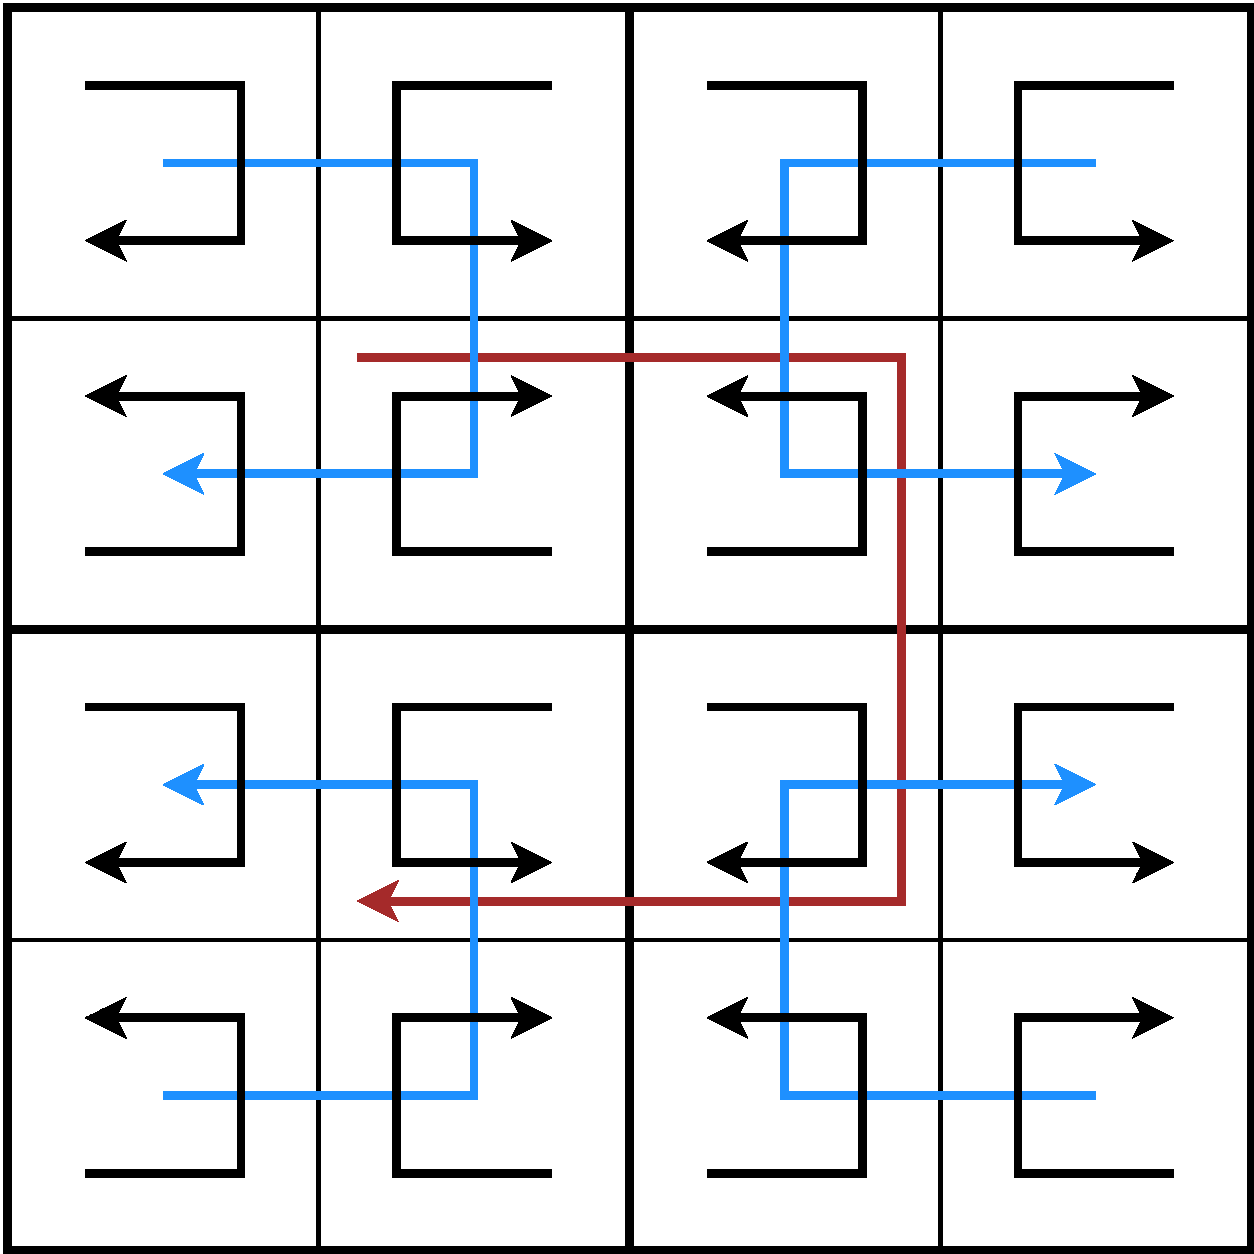
\includegraphics[width=\textwidth]{modgray-2-levels-arrows.pdf}
		\caption{}\label{fig:modgray-2-levels-arrows.pdf}
	\end{subfigure}%
	\quad
	\begin{subfigure}[c]{4.6cm}
		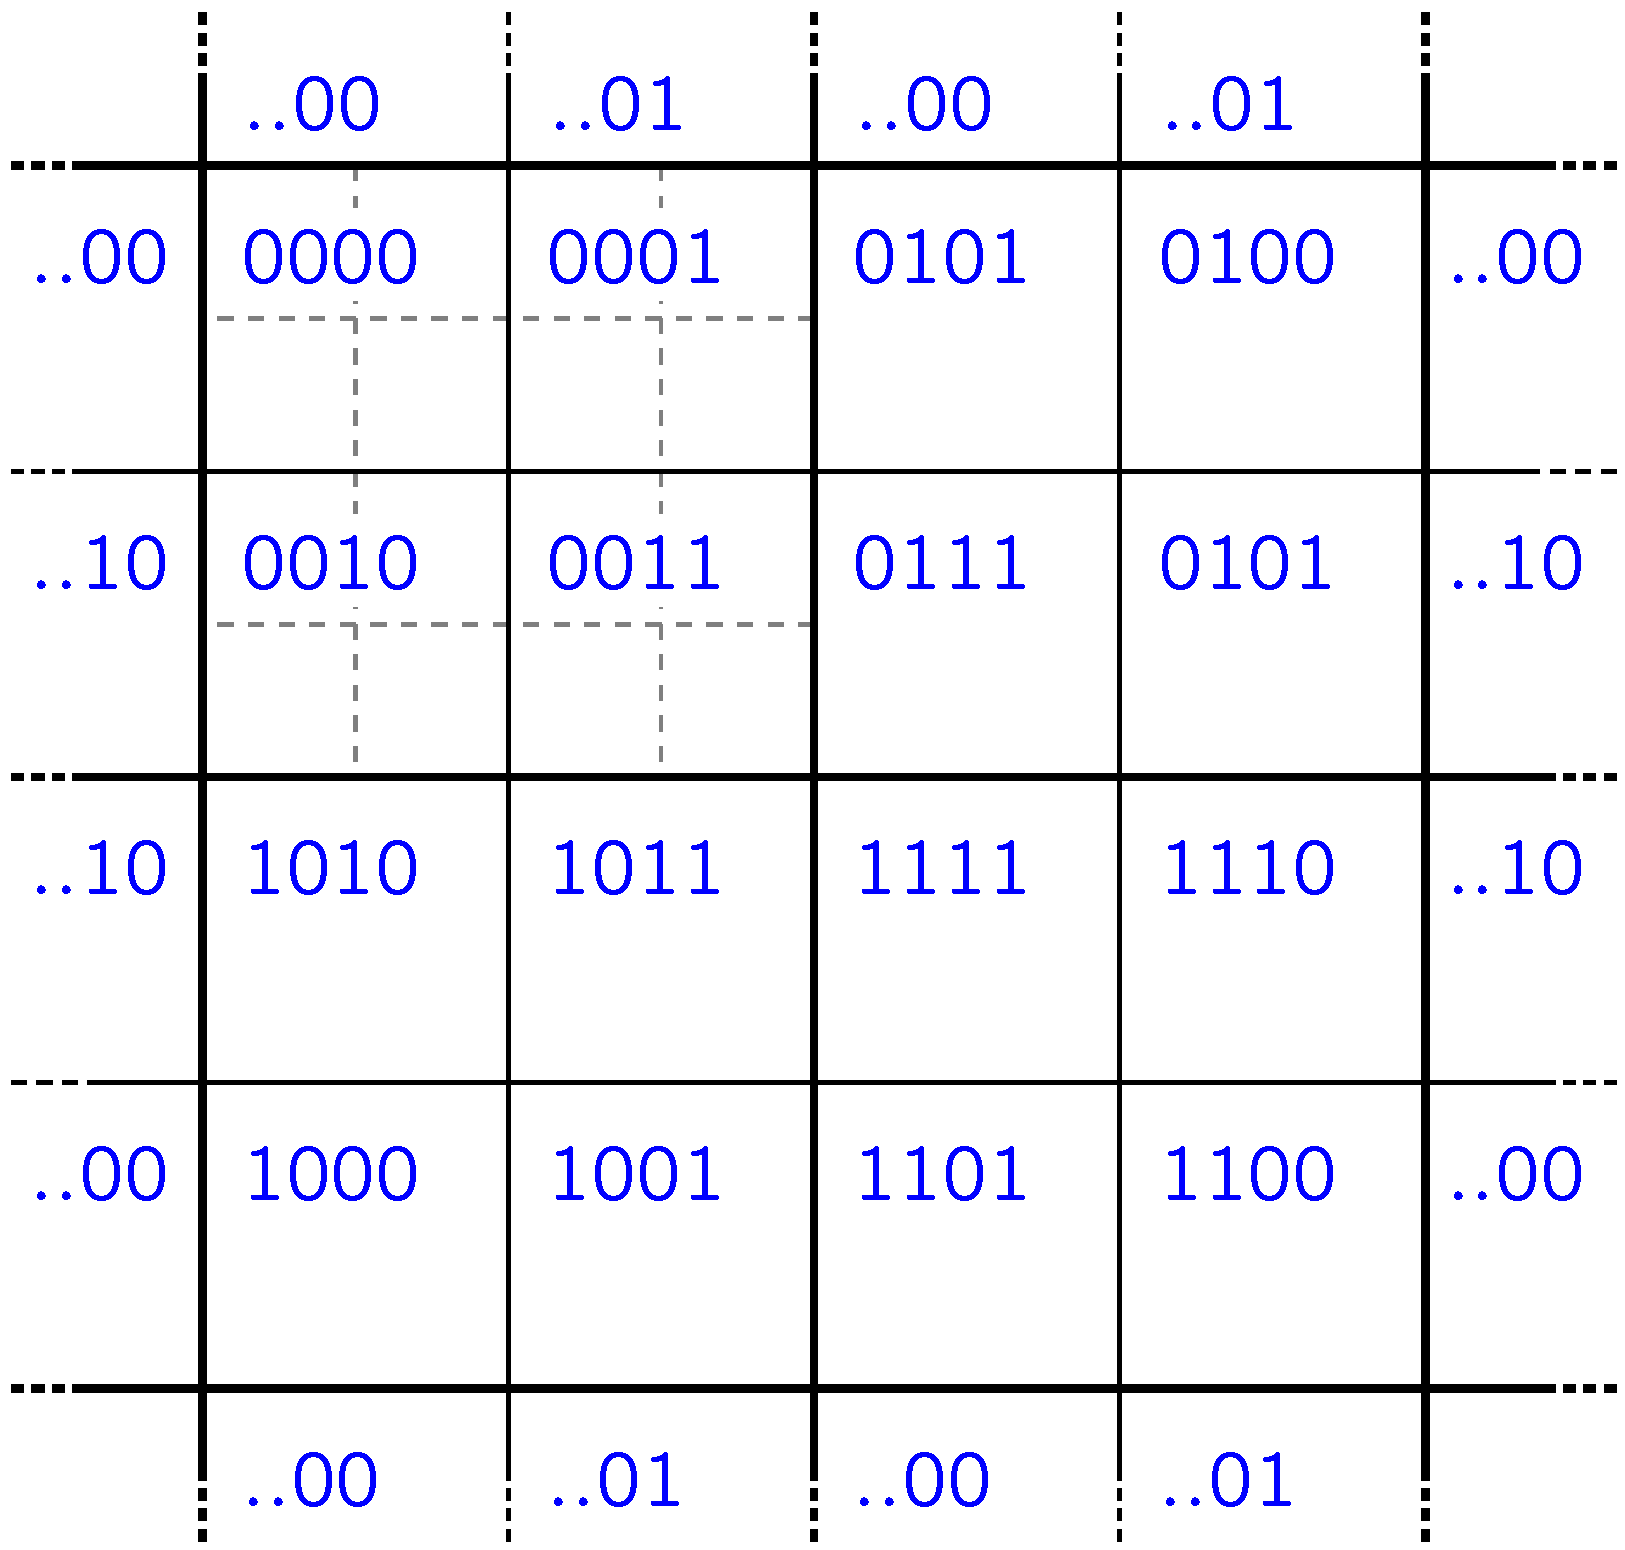
\includegraphics[width=\textwidth]{modgray-2-levels-numbers.pdf}
		\caption{}\label{fig:modgray-2-levels-numbers.pdf}
	\end{subfigure}

	\caption[Modified Gray Code ordering]{The tree traversal that was developed
		for this project is a variation of the Gray code order discussed in
		Section~\ref{ssub:gray_codes}.  Instead of all sub-quadrants having the
		same orientation, each is reflected in either the x- or y-axis,
		\subref{fig:modgray-2-levels-arrows.pdf}. This has the advantage that
		neighbouring nodes have codes which differ by exactly one bit,
		\subref{fig:modgray-2-levels-numbers.pdf}.}\label{fig:modgray-traversal}
\end{figure}

\begin{figure}[tbhp]
	\centering
	\includegraphics[width=7.4cm]{modgray-steps.pdf}
	%TODO short caption
	% TODO caption
	\caption{modgray-Steps}\label{fig:modgray-steps}
\end{figure}

\subsubsection{Other Orderings}
\label{ssub:other_orderings}

As well as the orderings discussed above, there are also a number of other
space filling curves and dis-joint orderings that were also discounted.
Figure~\ref{fig:modgray-2-alternatives} shows some of these.

\begin{itemize}

	\item Figure~\ref{fig:modgray-alt-order.pdf} shows \emph{row order}
		traversal of the grid. This extremely simple to implement for a simple
		grid-like arrangement, but is very awkward and looses much of the
		information when using quadtrees.

	\item Figure~\ref{fig:modgray-alt-prime.pdf} shows \emph{row-prime order},
		also known as snake-order\cite{goodchild1983optimizing}, traversal.
		This is a slight modification of row order which is continuous, again,
		is not recursive so not suitable for use with quadtrees.

	\item Figure~\ref{fig:modgray-alt-rotated.pdf} is identical to them
		modified Gray order above, but with a single \SI{90}{\degree} rotation.
		Since the orientation of an image has no effect on the clusters found,
		all rotations and reflections provide the same functionality as the
		original. The particular form chosen is simply due to {\ae}sthetic
		preference.

	\item Figure~\ref{fig:modgray-alt-pinwheel.pdf} shows an alteration to the
		modified Gray code order, named \emph{pinwheel order}, where, instead of
		reflecting the quadrants, each is rotated about it's center
		\SI{90}{\degree} so that the whole image is rotational symmetric,
		something the modified Gray code lacks.  This form turns out not to
		provide any additional features and makes conversion from quadtree code
		to coordinate representation substantially more difficult.

\end{itemize}

\begin{figure}[tbhp]
	\centering
	\begin{subfigure}[b]{3.5cm}
		\includegraphics[width=\textwidth]{modgray-alt-order.pdf}
		\caption{}\label{fig:modgray-alt-order.pdf}
	\end{subfigure}%
	\quad
	\begin{subfigure}[b]{3.5cm}
		\includegraphics[width=\textwidth]{modgray-alt-prime.pdf}
		\caption{}\label{fig:modgray-alt-prime.pdf}
	\end{subfigure}
	\\[0.2cm]
	\begin{subfigure}[b]{3.5cm}
		\includegraphics[width=\textwidth]{modgray-alt-rotated.pdf}
		\caption{}\label{fig:modgray-alt-rotated.pdf}
	\end{subfigure}%
	\quad
	\begin{subfigure}[b]{3.5cm}
		\includegraphics[width=\textwidth]{modgray-alt-pinwheel.pdf}
		\caption{}\label{fig:modgray-alt-pinwheel.pdf}
	\end{subfigure}

	\caption[Alternative quadtree orderings.]{There are a number of different
		space filling curves that can be used to map a two dimensional grid to
		a single dimensional array. To be considered for use in the quadtree
		ordering, the new ordering must provide some improvement of efficiency
		of some operations. Here are shown some orderings which were
		discounted.}\label{fig:modgray-2-alternatives}
\end{figure}

Since the quadtree is a recursive data structure, it is necessary to be able to
maintain the correct orientation of child trees with respect to their parents
at the construction stage. It turns out that this is easy to achieve and thus
adapting it for each of the arrangements discussed above is simply a matter of
adjusting the next part of the code that is added for each of the four children
when creating them. Pseudo code to achieve this for the Morton order and the
modified Gray code order is shown in Listings~\ref{code:child_construction}
and~\ref{code:child_construction_mgc}.

	%TODO short caption
\begin{lstlisting}[caption={Code to generate children of the current quadtree
while maintaining the correct ordering. Z- and Gray ordering.},
label=code:child_construction]
	// Constructor
	Quadtree(max_x, max_y, code)

	// Child creation,  Z-Order
	t_l = new Quadtree(100, 100, this.code + "00");
	t_r = new Quadtree(100, 100, this.code + "01");
	b_l = new Quadtree(100, 100, this.code + "11");
	b_r = new Quadtree(100, 100, this.code + "10");

	// Child creation,  Gray Code
	t_l = new Quadtree(100, 100, this.code + "00");
	t_r = new Quadtree(100, 100, this.code + "01");
	b_l = new Quadtree(100, 100, this.code + "10");
	b_r = new Quadtree(100, 100, this.code + "11");
\end{lstlisting}

	%TODO short caption
\begin{lstlisting}[caption={Code to generate children of the current quadtree
while maintaining the correct ordering. Modified Gray code order. Since the
ordering is different for each quadrant, the ordering is changed depending on
the position of the current node.},
label=code:child_construction_mgc]
	// Child creation, Modified Gray Code
	this.position = pos;
	if (pos == "tl") {
		new_code[0] = code + "00";
		new_code[1] = code + "01";
		new_code[2] = code + "10";
		new_code[3] = code + "11";

	} else if (pos == "tr") {
		new_code[0] = code + "01";
		new_code[1] = code + "00";
		new_code[2] = code + "11";
		new_code[3] = code + "10";

	} else if (pos == "bl") {
		new_code[0] = code + "10";
		new_code[1] = code + "11";
		new_code[2] = code + "00";
		new_code[3] = code + "01";

	} else if (pos == "br") {
		new_code[0] = code + "11";
		new_code[1] = code + "10";
		new_code[2] = code + "01";
		new_code[3] = code + "00";
	}

	t_l = new Quadtree(100, 100, this.code + new_code[0]);
	t_r = new Quadtree(100, 100, this.code + new_code[1]);
	b_l = new Quadtree(100, 100, this.code + new_code[2]);
	b_r = new Quadtree(100, 100, this.code + new_code[3]);
\end{lstlisting}

\subsection{Hash Table Implementation}
\label{sub:hash_table_implementation}

In order to speed up the subsequent operations applied to the quadtree
structure, it is converted to a simpler, one dimensional data structure. The
method discussed above, to number the cells in a logical fashion based on the
code of the parent, can be viewed as a way to map the two dimensional image to
a single unique binary code, and hence to a one dimensional format. Thus, the
quadtree can be easily converted to an array structure by simply using the key
code as the array index. Once this is performed the access complexity is
significantly reduced. This operation is only performed once after the quadtree
has been generated meaning the amortized complexity is reduced.

As mentioned in Part~\ref{prt:data_structures}, using a na\"{\i}ve
implementation has the potential to have a very poor space usage if the image
is not densely populated (in which case it is likely that few clusters would be
identifiable anyway). Instead, an implementation is created that makes use of
the \emph{Hash Table} data structure\cite{cormen2001introduction}. This allows
the data structure to increase in size dynamically as more space is needed, but
also provides linear time complexity for access, modification and search. The
quadtree code is used as the key for the hash table, and the data stored within
the cell with that code is the hash table value.

Using this data structure means that several operations are significantly sped
up. For example, for the quadtree format, the steps required to check if a
given code is present involves traversing the tree as specified by the code to
check and waiting to see if a node with that code is found, thus $O(\log n)$.
However, for a hash table, the hash function is used to get a hash of the code
to be checked and the appropriate location checked. If the codes match, then
the code does appear in the tree, a total of two operations, constant $O(1)$.

Also, since the structure is defined recursively, it is not possible to
directly access a given location of the data. Instead it must be arrived at by
starting at the root, and, for every level, deciding which of the children the
destination exists in. This would be a time consuming step for a number of
operations, but the biggest effect would be when checking the neighbours of
cells since for every neighbour of every node, the tree must be traversed. This
is not an issue for the hash table since the single dimensional nature means
that data can be accessed anywhere directly.

Little spatial information should be lost during the conversion from quadtree
to hash table since this is all contained in the quadtree code assigned to the
node during the quadtree generation step. However, the quadtree representation
can be kept in memory for some processes. For example, to get all of the leaf
nodes of a given node, it is enough to start at that node and traverse the tree
in post- or pre-order and return the nodes that are arrived at, $O(\log n)$,
whereas, for the hash table, each node must be checked to decide if it is a
child, $O(n)$.

A hash table requires two pieces of information for each entry: a \emph{key}
and a \emph{value}. The key is what is used to locate items, its hash is used
as the index of the array used internally. The value is the information that
should be accessible when using the key. For this application, since more than
a single piece of information should be accessible for each quadtree code, an
object is stored against each key. This has the format shown in
Table~\ref{tab:hashmap-columns}.

\begin{table}[htbp]
	\centering
	\begin{tabu}{l X}
		\toprule
		Key  & Value \\
		\midrule
		Quadtree Code & $\bullet$ Set of points in this node \\
					&	$\bullet$ Cluster these points exist in \\
					&	$\bullet$ Size of this node \\
					&	$\bullet$ Number of edges this node contributes to
		the perimeter of the cluster\\
		\bottomrule
	\end{tabu}

	% TODO caption
	\caption{}\label{tab:hashmap-columns}
\end{table}

% Created:  Thu 10 Jul 2014 04:22 PM
% Author:   Josh Wainwright
% Filename: quadtree-traversal.tex

\section{Quadtree Traversal}
\label{sec:quadtree_traversal}

Whether the quadtree is stored in memory as a recursive quadtree data
structure, or as hash table, Section~\ref{sub:hash_table_implementation}, the
most important and computationally intensive step is extracting the clusters at
the correct depth and disregarding those data points that can be attributed to
noise.

The quadtree numbering system chosen lends itself very well to analysis based
on spatial location and the proximity of neighbours to a given node being
examined.

\subsection{Algorithm Description}
\label{sub:algorithm_description}

To \emph{propagate} is defined as the act of ``spreading and promoting (an
idea, theory etc.) widely''\cite{oed31}. This term shall refer to the process
by which a single starting location, previously chosen, is expanded by
examining neighbours to form a cluster. The algorithm is defined recursively
with the main step being `propagation' of nodes. The propagation algorithm is
performed as follows:

\begin{enumerate}
	\item Choose a starting location that has not yet been checked, $l$.
	\item For this given starting location, the $i$ neighbours surrounding it,
		$n_0$ to $n_i$, are checked for validity based on the conditions of the
		analysis (the way these neighbours are selected is discussed in
		Section~\ref{sub:choosing_neighbours}).
	\item If a node fails the check, then it is recorded as having done so and
		shall not be checked again. If it passes, then it is, itself,
		propagated.
		\begin{itemize}
			\item To be ``propagated'' means to perform this propagation
				algorithm using that node as the starting location.
		\end{itemize}
	\item When all nodes have been checked, return to step 1.
	\item The algorithm completes either when;
	\begin{itemize}
		\item every one of the nodes in the image have been checked and
			included or ignored, or
		\item the cluster has ended, so all the neighbours of all checked nodes
			have failed the validity tests and no further starting locations
			were found or specified.
	\end{itemize}
\end{enumerate}

This process is shown graphically in Figure~\ref{fig:propogation}.

\begin{figure}[tbh]
	\centering
	\includegraphics[width=7cm]{propogation.pdf}

	\caption[Propagation of a cluster from a starting location.]{For a starting
		location, (a), in an image, no information is known and so all its
		neighbours are checked. Some of these are found to be part of the
		cluster, others are rejected. The ones that are included are then,
		themselves, checked and so on. As the cluster grows, (b), (c) and
		(d), the number of checked nodes increases.}\label{fig:propogation}
\end{figure}

Listing~\ref{code:quadtree-propagate} shows pseudo code for the propagate
algorithm which, starting at a given starting location, expands the cluster
outwards while there still exist valid neighbours that should be included. The
\texttt{getNeighbours()} method is described in
Section~\ref{sub:choosing_neighbours}. This is a recursively defined algorithm
which calls itself for each of the neighbours of a node and for each of their
neighbours, and so on. There is a condition that prevents the algorithm from
being called again on nodes that have been checked already. This prevents a
loop from forming and preventing the algorithm terminating.

\begin{center}
\begin{minipage}{\textwidth}
\begin{lstlisting}[caption={[Code for the propagate algorithm.]Code for the
	propagate algorithm which expands an initial starting location to a
	cluster.}, label=code:quadtree-propagate]
	function |propagate()| {
		node[] startLocations = getStartLocations() (*@\label{eql:a}@*)
		for each node in startLocations
			propagate(node)
	}

	function |propagate(node)| {
		if (not node.inCluster()) (*@\label{eql:b}@*)
			node[] neighbours = getNeighbours(node)

			for each n in neighbours  (*@\label{eql:c}@*)
				if (n is valid) propagate(n)
	}
\end{lstlisting}
\end{minipage}
\end{center}

In reference to Listing~\ref{code:quadtree-propagate} above:
\begin{description}
	\item[Line~\ref{eql:a}] A set of starting locations is selected based on
		some heuristic that determines if a node is deep enough in the tree to
		be used as a starting location.

	\item[Line~\ref{eql:b}] Nodes are only propagated if they have not already
		been included in a cluster. If this were not the case, then clusters
		would overlap.

	\item[Line~\ref{eql:c}] Each of the neighbours of the current node is
		propagated. The method of choosing neighbours determines how far the
		cluster can spread, and is separated from the clustering algorithm.
\end{description}

When discovering clusters via this propagation technique, care must be taken to
avoid a run-away situation where every node in the tree gets included. This
would happen when looking at the neighbours of a node and blindly including
them. Since every internal node has exactly four neighbours, the propagation
would terminate only when reaching the boundary nodes. Instead, the depth of
the node must be considered. Again, the simplest method is not sufficient. If
the propagation is limited to a given node depth, even if this is not the same
as the deepest node, the size of any clusters that are identified will be
limited, as shown in Figure~\ref{fig:propogation-halting}.  Since the depth to
consider is not able to change, when the neighbours of the blue node are
checked, no correct neighbours are found and so the process terminates. When
able to view the larger structure of the nodes, however, it is clear that the
structure continues beyond the gap, following the dotted line.

\begin{figure}[tbh]
	\centering
	\begin{subfigure}[c]{5.2cm}
		\includegraphics[width=\linewidth]{propogation-halting.pdf}
		\caption{}\label{fig:propogation-halting}
	\end{subfigure}%
	\quad
	\begin{subfigure}[c]{3.2cm}
		\includegraphics[width=\linewidth]{propogation-levels.pdf}
		\caption{}\label{fig:propogation-levels}
	\end{subfigure}

	\caption[Considerations regarding quadtree levels to be accepted.]
		{Considerations regarding quadtree levels that will be accepted
		when propagating a node in a quadtree. \subref{fig:propogation-halting}
		If the depth range that specifies how far up the tree to look for valid
		neighbours is too small then a cluster might be terminated too soon.
		\subref{fig:propogation-levels}(i) a depth range of two and, (ii) a
		depth range of three.}\label{fig:prop-levels-halting}
\end{figure}

To avoid this, a certain amount of leniency must be allowed when deciding what
constitutes a neighbour. Given an appropriate value, this would allow both of
the larger white cells in Figure~\ref{fig:propogation-halting} to be included.

The term \emph{depth range} shall define the levels that are to be considered
when choosing neighbours with respect to a target depth. Since clusters are
being considered as areas of increased density of points, all cells with a
depth greater than the target depth shall be allowed, so the purple cells in
Figure~\ref{fig:propogation-halting} would be included when the target depth is
the same as the depth of the included red cells. A depth range of zero is
equivalent to the situation above where only cells of a given depth are
considered. A depth range of one would mean that the white square in
Figure~\ref{fig:propogation-levels}\,(i) would be included but not in~(ii),
whereas a depth range of two would include both and so on.

\subsection{Clustering Start Locations}
\label{sub:clustering_start_locations}

In order for the algorithm to proceed correctly, a good initial node, a
starting location, must be chosen. Since the clusters to be found are regions
of high point density, it makes sense to start the clustering algorithm at the
point in the image with the highest point density. This should ensure that the
most defined cluster is always found with subsequent clusters being less dense,
and so less well defined.

When starting at the highest density node, i.e., the node which is at the
deepest level in the tree, propagating this node and then terminating; the
cluster shown in Figure~\ref{fig:single-cluster} is found. The file
\texttt{palm-1.txt} was used and generated this data in
\SI{457}{\milli\second}. This shows that the algorithm works correctly.
Altering the parameters that are used to generate the quadtree affects the size
of the nodes that are included in the cluster and the depth that is searched.

\begin{figure}[tbh]
	\centering
	\begin{subfigure}[c]{4.2cm}
		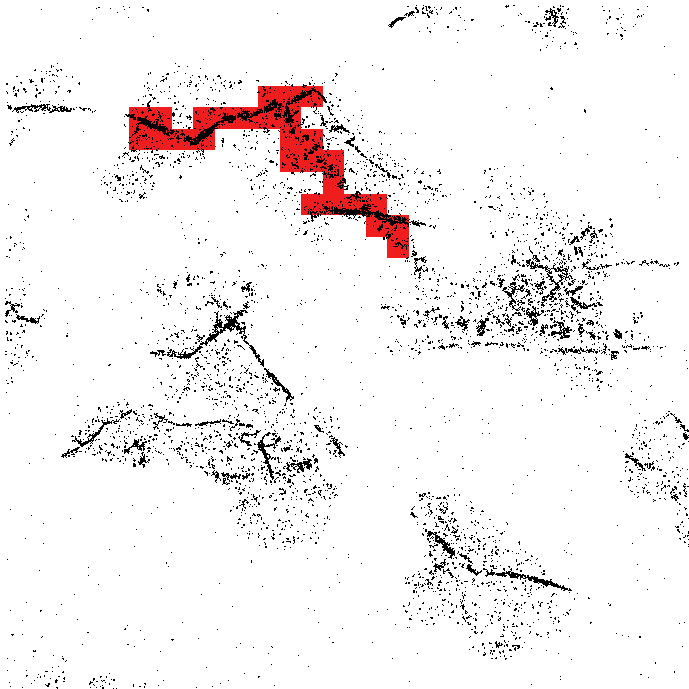
\includegraphics[width=\textwidth]{single-cluster.png}
		\caption{}\label{fig:single-cluster-points}
	\end{subfigure}%
	\quad
	\begin{subfigure}[c]{4.2cm}
		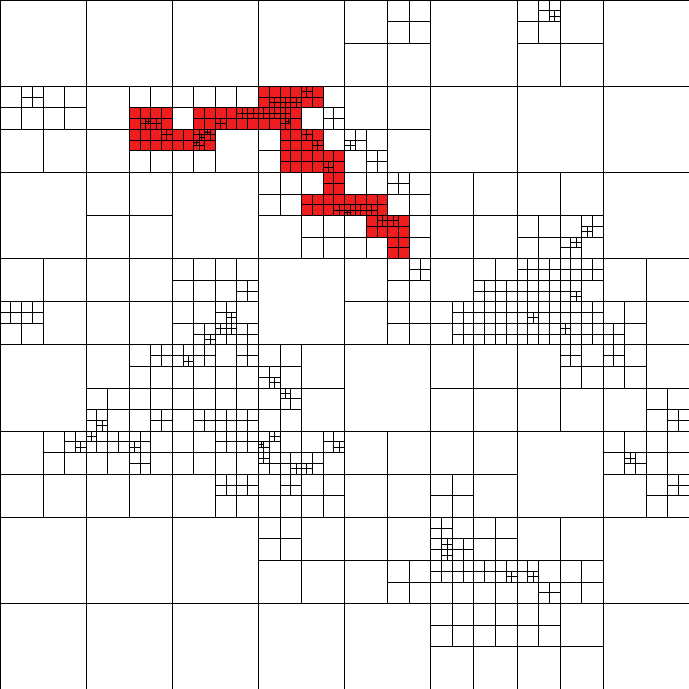
\includegraphics[width=\textwidth]{single-cluster-lines.png}
		\caption{}\label{fig:single-cluster-lines}
	\end{subfigure}

	\caption[Propagation of a single starting location.]{Initial versions of
		the clustering algorithm terminated immediately after finishing
		propagating the first cluster. This gives a useful test as to the
		correctness of the algorithm since there are no other clusters for this
		to collide with. It is useful to be able to check both
		\subref{fig:single-cluster-points} the points that were considered to
		be in the cluster and \subref{fig:single-cluster-lines} the nodes in
		the quadtree that were included and where the propagating algorithm
		stopped.}\label{fig:single-cluster}
\end{figure}

In order to find other clusters, the algorithm must be restarted with a new
starting location. This is chosen as the deepest node in the tree that is not
already included in a cluster. There are a number of different way to terminate
this process of finding new clusters:

\begin{itemize}

	\item Perform a set number of iterations. This performs well if the
		clusters to be located can be easily counted, but in the general case,
		this is not possible or desired. If the number of iterations is set to
		a high value, of the order of 50, the algorithm will continue to locate
		``clusters'' even if they do not exist and will eventually simply
		report the background noise as a cluster. To prevent this, a limit can
		be set on the depth a starting location must be in order to be valid.

	\item Continue iterating until a depth limit is reached. This is a more
		general form of the previous case, but for this case, the limit on the
		depth of a starting location will always be reached.

	\item Allow the user to make a number of starting point location selections
		manually. Since ImageJ allows multi-point region of interest (ROI)
		selections, the user could be asked to place a new ROI at the places
		they consider a reasonable place to find a cluster. The algorithm would
		then convert the locations of each of these ROI points into the
		relevant quadtree code and begin propagating from that node and
		terminate when all of the ROI's had been used. This suffers from the
		same issues as method 1, since it is not helpful to require the user to
		make the selections manually.

\end{itemize}

The plugin developed uses a combination of the first and second approaches.
Since the number of clusters cannot often be counted easily, the user cannot be
expected to provide this value. However, it is also very difficult to determine
when clusters that are being propagated are valid or not. The algorithm can be
instructed to halt if the nodes that are being considered are too high up the
tree, i.e., too many nodes have been included and the algorithm has run away,
but this is generally not sufficient for all cases. Instead, a comparison with
the depth range allowed (which is set by the user) with the difference between
the first cluster found and the current cluster is made. If the difference is
similar to the depth range, then the algorithm continues. After this process
has finished, the clusters that have been found are examined and those that are
too small with respect to the others are removed.

\begin{figure}[tbh]
	\centering
	\begin{minipage}[c]{7cm}
		\fbox{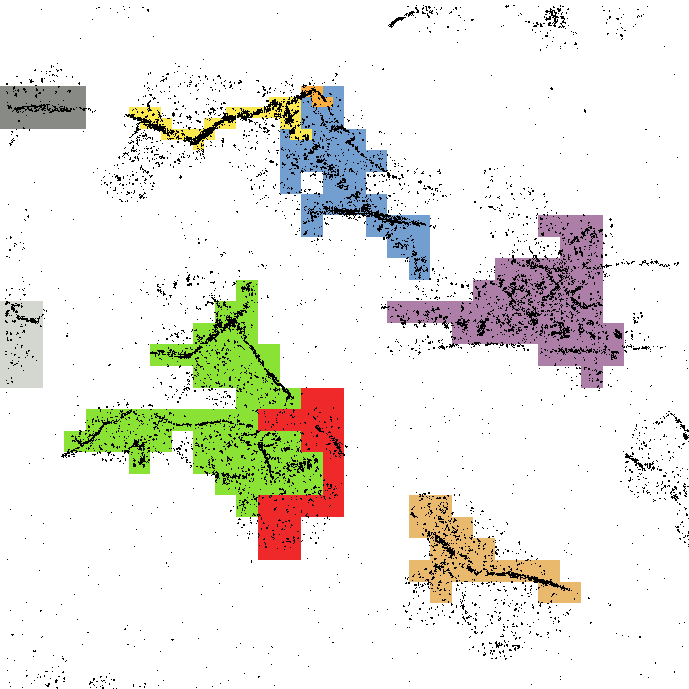
\includegraphics[width=\textwidth]{multiple-clusters-colours.png}}
	\end{minipage}%
	\,
	\begin{minipage}[c]{1cm}
		\centering
		\begin{tabular}[b]{l}
			\cellcolor{lyellow}1 \\
			\cellcolor{lorange}2 \\
			\cellcolor{lbrown}3 \\
			\cellcolor{lgreen}4 \\
			\cellcolor{lblue}5 \\
			\cellcolor{lpurple}6 \\
			\cellcolor{lred}7 \\
			\cellcolor{silver}8 \\
			\cellcolor{lgrey}9 \\
		\end{tabular}
	\end{minipage}

	\caption[Propagation of multiple starting locations.]{Initial versions of
		the clustering algorithm included too many nodes, making the clusters
		too large. This image shows how each node cluster that is started is
		independent of the previous ones. The clusters were identified in the
		order they are listed on the right.}\label{fig:multiple-clusters-colours}
\end{figure}

\subsection{Choosing Neighbours}
\label{sub:choosing_neighbours}

Some care must be taken when deciding what constitutes a neighbour of a node
and what does not. As mentioned above, when detecting clusters using
propagation, the neighbours of a node are checked and, if they are valid, are
themselves propagated. For this reason, a poor choice of neighbours means that
the propagation will either:

\begin{itemize}
	\item be cut short too early, and so not all of the clusters will be
		located, or
	\item include too many nodes, in which case the clusters will not represent
		the actual data.
\end{itemize}

The first neighbours that must be considered, named \emph{rook's case}
% TODO remove brackets around citation
neighbours by~\cite{abel1990comparative}, are the four nodes that lie to the
north, east, south and west of the current node. These are the nodes that are
directly in contact with the node and so, if they are valid, represent a direct
continuation of the cluster.

However, if the choice of neighbours is limited to these four, some major
structures are missed. Figure~\ref{fig:kernel-rooks-case} shows how this
arrangement misses a large portion of the cluster, simply because the
propagation could not consider the nodes across the boundary. If, in addition
to the rook's case, the four \emph{diagonal} neighbours are included, giving a
total of eight, the results are much more complete, as shown in
Figure~\ref{fig:kernel-all8}.

\begin{figure}[tbh]
	\centering
	\begin{subfigure}[b]{4.2cm}
		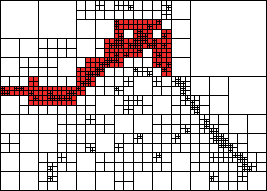
\includegraphics[width=\textwidth]{clusters/kernel-rooks-case.png}
		\caption{}\label{fig:kernel-rooks-case}
	\end{subfigure}%
	\quad
	\begin{subfigure}[b]{4.2cm}
		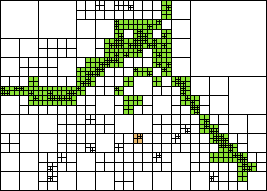
\includegraphics[width=\textwidth]{clusters/kernel-all8.png}
		\caption{}\label{fig:kernel-all8}
	\end{subfigure}

	\caption[A comparison of different neighbour sets.]{A comparison between
		different neighbour sets.  \subref{fig:kernel-rooks-case} shows how
		some of the cluster is lost when using just the rook's case neighbours,
		whereas, using all eight neighbours, Figure~\subref{fig:kernel-all8}
		more of the cluster is included.}\label{fig:kernel-options}
\end{figure}

\subsubsection{Image Kernel}
\label{ssub:Image Kernel}

The requirement to include eight neighbours for each node suggests that it
might be of value to allow users to specify an arbitrary number of neighbours
around the given cell.

In many applications in image processing, the concept of an image \emph{kernel}
is commonplace. This is a square, odd-sided matrix that is used to apply
filters and other effects to an image. The kernel is placed over each of the
pixels in the image in turn so that the central element in the matrix is over
the current pixel and each of the other elements is over another pixel. The
value of the element in the kernel is then used to manipulate the pixels in the
image below it. For example, to blur an image, a $3\times 3$ kernel composed of
all $\rfrac{1}{9}$'s can be used. When applied, this would mean that the
% TODO reread sentence
current pixel is given a value which is the sum of each of matrix elements
multiplied by the pixel value beneath it.

A similar technique is used here to choose neighbours from the quadtree. The
image kernel that is used is a binary matrix, meaning that all of the elements
are restricted to either 0 or 1, but, in all other respects, is the same as a
regular image kernel. The kernel is placed over a node of interest. Any node
that lies under an element with a value of 1 is included as a neighbour and
nodes under 0 elements are ignored. The value of the central element in the
kernel does not matter, but the convention is to set this to 1.

Thus, the simplest kernel, though of least use, is the identity kernel which
has an element with value `1' in the centre and all other elements `0',
Figure~\ref{fig:kernel-identity}. This would result in no neighbours being
selected, and so no clusters located. The rook's case neighbours are now
represented with the kernel in Figure~\ref{fig:kernel-image-rooks} and the case
with all 8 neighbours in Figure~\ref{fig:kernel-image-all8}.

\begin{figure}[tbh]
	\centering
	\begin{subtable}[b]{0.2\textwidth}
	\centering
		\begin{tabular}{|l|l|l|}
			\hline
			0 & 0 & 0 \\
			\hline
			0 & \cellcolor{lred}1 & 0 \\
			\hline
			0 & 0 & 0 \\
			\hline
		\end{tabular}
		\caption{}\label{fig:kernel-identity}
	\end{subtable}%
	\quad
	\begin{subtable}[b]{0.2\textwidth}
	\centering
		\begin{tabular}{|l|l|l|}
			\hline
			0 & 1 & 0 \\
			\hline
			1 & \cellcolor{lred}1 & 1 \\
			\hline
			0 & 1 & 0 \\
			\hline
		\end{tabular}
		\caption{}\label{fig:kernel-image-rooks}
	\end{subtable}%
	\quad
	\begin{subtable}[b]{0.2\textwidth}
	\centering
		\begin{tabular}{|l|l|l|}
			\hline
			1 & 1 & 1 \\
			\hline
			1 & \cellcolor{lred}1 & 1 \\
			\hline
			1 & 1 & 1 \\
			\hline
		\end{tabular}
		\caption{}\label{fig:kernel-image-all8}
	\end{subtable}

	\caption[Kernels for the identity matrix, rook's case and all 8
		neighbours.]{Kernels for~\subref{fig:kernel-identity} the identity
		matrix,\subref{fig:kernel-image-rooks} rook's case neighbours
		and~\subref{fig:kernel-all8} all 8 neighbours. The central cell of the
		kernel can be anything as it is never included as a neighbour.}\label{fig:kernel-neighbours}
\end{figure}

This functionality provides the ability to target certain types of clusters
depending on the spatial orientation of the cluster; vertical or horizontal
etc. Figure~\ref{fig:kernel-shapes} shows a number of possible kernel shapes
that would allow different types of clusters to be targeted. Each of these show
the central cell with the cells that would be represented by a 1; cells
represented by 0's are not displayed.

\begin{figure}[tbh]
	\centering
	\includegraphics[width=7cm]{kernel-shapes.pdf}

	\caption[Different kernel shapes for different clusters.]{Different kernel
		shapes can be used to find different sorts of clusters. (a)~The basic
		rook's case neighbours and (b)~the full number of closest neighbours
		are the simplest general cases, used for most clusters. (c)~The area to
		search can be extended by including more neighbours---this could help
		find clusters that are more sparsely populated. Clusters of a specific
		orientation can be located, for example, predominately (d)~vertical or
		(e)~NW SE diagonal.}\label{fig:kernel-shapes}
\end{figure}

\subsubsection{Searching Up and Down the Tree}
\label{ssub:searching_up_and_down_the_tree}

Once a node location has been identified as a valid neighbour, there is still
no guarantee that there exists a node there. There are three possible cases
concerning the location that has been identified. Each of these situations must
be handled differently in order to ensure that all of the correct nodes are
selected as neighbours.

\begin{enumerate}
	\item The location represents a leaf node, in which case the process is
		complete and a neighbour has been identified,
		Figure~\ref{fig:updownsearch}a.

		In this case, no further action must be taken.

	\item The location is to be a non-existent node, i.e., there may be a leaf
		node at a position further up the tree than the location meaning there
		is nothing at this position in the tree,
		Figure~\ref{fig:updownsearch}b.

		In this case, either the code that has been obtained from the kernel
		analysis must be shortened until it represents a node that exists in
		the tree, or the tree must be traversed according to the quadtree code
		until a leaf node is reached. The located node must then be compared
		against the node to which this is a neighbour to check that the two are
		within the depth range specified (Section~\ref{sub:option_sliders}).

	\item The location is a node in the quadtree which is not a leaf node,
		i.e., it has four children, each of which may be trees or leaves,
		Figure~\ref{fig:updownsearch}c.

		For this third case, the depth range is not considered since all nodes
		deeper than the starting node are assumed to be a part of the same
		cluster. Instead, all leaf nodes below the node represented by the code
		are included as valid neighbours, and hence are, themselves,
		propagated. To get these children, the sub-tree below the current node
		is traversed in pre- or post-order and every leaf node that is
		encountered is added as a neighbour.

\end{enumerate}

\begin{figure}[tbh]
	\centering
	\includegraphics[width=5cm]{updownsearch.pdf}
	\caption[Possible results of neighbour selection.]{The possible results of
		neighbour selection. The blue square is the node that is being
		propagated and the red square represents the location of the node given
		by the neighbour code, black squares are real nodes in the tree. (a)
		shows the ideal case where the neighbour is a node, (b) shows where the
		code could be further down in the tree than exists and (c) shows the
		case where a real node is selected, but is not a leaf.}\label{fig:updownsearch}
\end{figure}

% Created:  TIMESTAMP
% Modified: TIMESTAMP

\section{ImageJ Plugin}
\label{sec:imagej_plugin}

\subsection{ImageJ}
\label{sub:imagej}

Imagej is an public domain, Java based image manipulation program written and
maintained by developers at the National Institute of Health. It is widly used
in medical and biological research and has an open API to allow extension via
macros, plugins and scripts.

Since they offer significantly betting integration, meaning speed and
efficiency improvements, a plugin is chosen to inegrate this project into
ImageJ over macros, which suffer performace loss when more than a few steps are
involved, and scripts which do not offer such tight integration with the rest of
the program.

The plugin shall allow a user to load a data set, as gathered from STORM, PALM
or similar imaging techniques discussed in
Section~\ref{sec:sub_diffraction_limit_imaging}, analyse the data for clusters
and receive detailed information regarding the clusters that were found.

% Created:  Fri 04 Jul 2014 04:47 PM
% Modified: Fri 11 Jul 2014 11:15 AM
% @author Josh Wainwright
% File name : imagej_plugin.tex

\section{ImageJ Plugin}
\label{sec:imagej_plugin}

The first version of the plugin simply allowed the user to visualise the data,
once it had been processed and entered into a quadtree. Though this provided
little benefit to the researcher producing data, it can be a useful tool to get
an insight into the process that a program is using to analyse one's data so
that the results can be better interpretted. For this reason, this version
served as a foundation for later versions of the plugin so that, when loading
data, a user gets the opportunity to view the data before proceding with the
analysis.

Again, earlier versions of the program displayed this data using the built-in
GUI classes in the AWT and Swing libraries included in the standard Java
distribution. This effectively prohibitted any further actions being performed
on the image once it had been generated since what was displayed was only
modifiable by the JVM via compiled code. It was also very memory intensive
since, in many cases, many thousands of separate objects (data points
represented by zero lenght lines, quadtree cells by boxes, etc) and so was slow
to draw initially and redraw with any subsequent move or resize of the window.

The code used to generate this view of the data was modified to make use of the
easy image generation functions present in ImageJ. Now, instead of many
different objects being manipulated for each view of the data, a single array
with a value for each pixel is needed. For the cases where the user wishes to
view the clusters that have been found, but not have them affect the image, the
image is created with a number of different \emph{slices} in the image
\emph{stack}. Slices are ImageJ's representation of images with two or more
layers, or alternative views, each of which resides in a stack of slices. Each
slice in a stack must have the same dimensions.

\begin{figure}[tbhp]
	\centering
	\includegraphics[width=0.8\linewidth]{imagej-stacks.pdf}
	\caption{imagej-Stacks}
	\label{fig:imagej-stacks}
\end{figure}

\begin{figure}[tbhp]
	\centering
	\begin{subfigure}[c]{0.48\linewidth}
		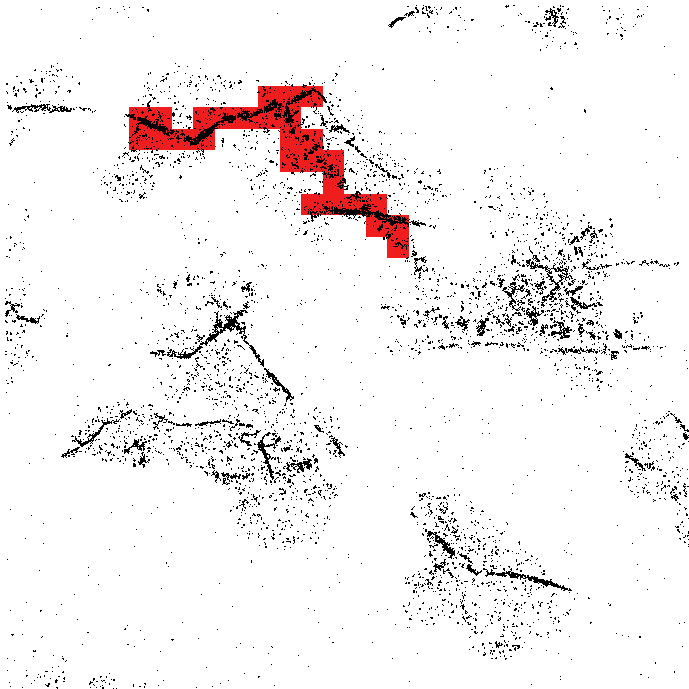
\includegraphics[width=\textwidth]{single-cluster.png}
		\caption{}\label{fig:single-cluster-points}
	\end{subfigure}%
	\quad
	\begin{subfigure}[c]{0.48\linewidth}
		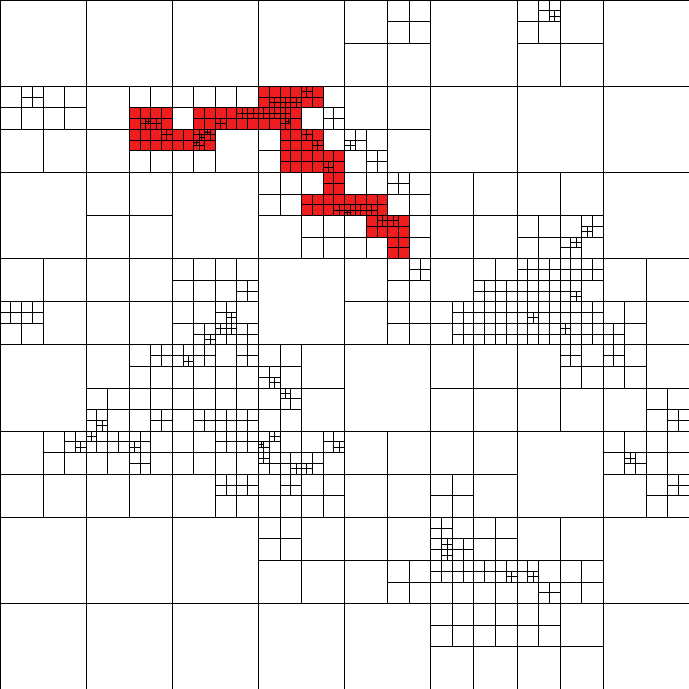
\includegraphics[width=\textwidth]{single-cluster-lines.png}
		\caption{}\label{fig:single-cluster-lines}
	\end{subfigure}
	% TODO caption
	\caption{} \label{fig:single-cluster}
\end{figure}

\begin{figure}[tbhp]
	\begin{minipage}[b]{0.85\linewidth}
		\centering
		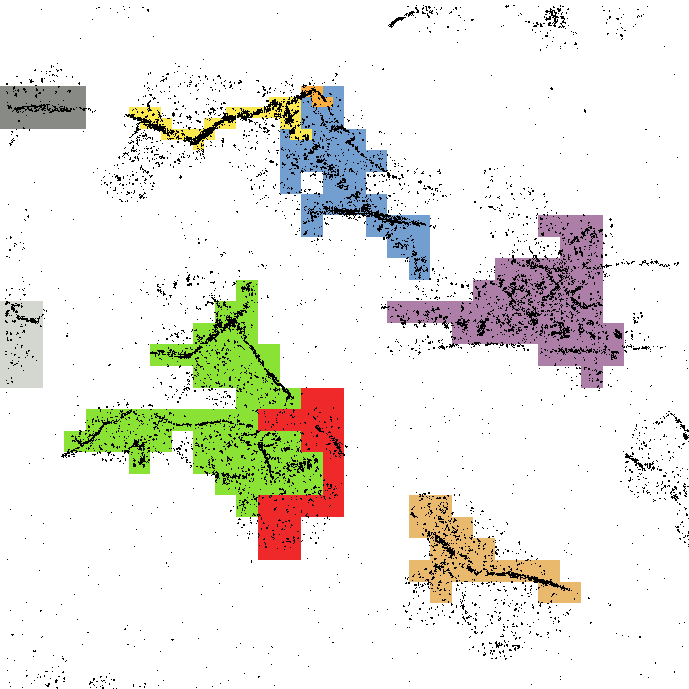
\includegraphics[width=\textwidth]{multiple-clusters-colours.png}
	\end{minipage}%
	\begin{minipage}[b]{0.1\linewidth}
		\centering
		\begin{tabular}[b]{ l l }
			\cellcolor[HTML]{FCE94F}1\\
			\cellcolor[HTML]{FCAF3E}2\\
			\cellcolor[HTML]{E9B96E}3\\
			\cellcolor[HTML]{8AE234}4\\
			\cellcolor[HTML]{729FCF}5\\
			\cellcolor[HTML]{AD7FA8}6\\
			\cellcolor[HTML]{EF2929}7\\
			\cellcolor[HTML]{D3D7CF}8\\
			\cellcolor[HTML]{888A85}9\\
		\end{tabular}
	\end{minipage}
	\caption{Bla bla}
	\label{fig:multiple-clusters-colours.png}
\end{figure}

% #fce94f
% #fcaf3e
% #e9b96e
% #8ae234
% #729fcf
% #ad7fa8
% #ef2929
% #d3d7cf
% #888a85

% Created:  Fri 01 Aug 2014 02:02 PM
% @author Josh Wainwright
% filename: analysis.tex

\section{Cluster Analysis}
\label{sec:cluster_analysis}

Once the data has been processed and a number of clusters have been identified,
they can be displayed on screen in an image to verify what was found and
perform further analysis. However, since the data that was used to find the
clusters is still held in memory at this point, it is useful to take advantage
of this and perform some immediate analysis and provide some statistics
regarding the clusters that were found.

There are two ways of conceptually viewing the clusters which will lead to
slightly different results when analysing them.

\begin{itemize}

	\item The first is to consider the boundary of the nodes of the quadtree
		that were considered to be part of a cluster to be the boundary of the
		cluster. This will mean that the actual cluster is likely to be
		slightly larger than the actual data points that it is comprised of,
		but is computationally simple to achieve, so fast, and can take into
		account any holes in the cluster.

	\item The second way is to, once the cluster has been located, discard the
		information about the nodes themselves, and simply use them to select
		the appropriate points. This results in a set of points that are all
		considered to be spatially grouped into the same cluster. From this
		set, calculations can be performed on the real data. This method is
		guaranteed to provide information that more closely represents the
		original data, though is more computationally intensive.

\end{itemize}

\subsection{Quadtree Node Analysis}
\label{sub:quadtree_node_analysis}

Here, the nodes of the quadtree that were considered part of the cluster are
considered, rather than the points that they contain.

\subsubsection{Cluster Area}
\label{ssub:cluster_area_node}

To calculate the area of the clusters, each node in each cluster is examined.
Since the size of the node must be known, it is calculated from the quadtree
code for that node. The formula is shown in Equation~\ref{eq:node-area},
\begin{align}
	a &= \frac{1}{4^{d}} \\
	a_i &= 4^{-l_i/2}, \label{eq:node-area}
\end{align}
where $a_i$ is the area of the node $i$, $d$ is the depth in the quadtree and
$l_i$ is the length of the quadtree code of that node. For every node in the
cluster, where there are $n$ nodes, this value is summed to give the total
cluster area, $A$:
\begin{align}
	A &= \sum_{i=0}^{n} a_i.
\end{align}

\subsubsection{Cluster Perimeter}
\label{ssub:cluster_perimeter_node}

Similarly to the cluster area, the perimeter is given as a fractional value of
the length of one side of the whole image, as calculated for each node from the
quadtree code, as shown in Equation~\ref{eq:node-perimeter},
\begin{align}
	p &= \frac{1}{2^{d}} \\
	p_i &= 2^{-l_i/2}, \label{eq:node-perimeter}
\end{align}
where the symbols have the same meaning as above.

However, this simply gives the length of one side of the node for any node. In
order to calculate the perimeter of the cluster, it is not enough to simply
sum these values, as for the cluster area, since not all nodes contribute to
the perimeter. Instead, for each node, it must be decided whether it
contributes to the perimeter and how much (1, 2, 3 or 4 sides), and then
increase the total perimeter by this many times the length of one side. The
total perimeter, $P$, then is given by Equation~\ref{eq:total-perimeter},
\begin{align}
	P &= \sum_{i=0}^{n} s * p_i, \label{eq:total-perimeter}
\end{align}
where $s \in \{0..4\}$. This is demonstrated in
Figure~\ref{fig:perimeter-edges} where the perimeter is simple to calculate in
case (a) as the nodes are all the same, but the size of each node must be taken
into account in case (b).

\begin{figure}[tbhp]
	\centering
	\begin{subfigure}[c]{3.5cm}
		\includegraphics[width=\textwidth]{perimeter-edges-grid.pdf}
		\caption{}\label{fig:perimeter-edges-grid.pdf}
	\end{subfigure}%
	\quad
	\begin{subfigure}[c]{3.5cm}
		\includegraphics[width=\textwidth]{perimeter-edges-quadtree.pdf}
		\caption{}\label{fig:perimeter-edges-quadtree.pdf}
	\end{subfigure}

	\caption[Perimeter size from node edge size.]{When calculating the
		perimeter of a cluster using the nodes that contribute, the size of
		each node must be taken into account. In
		case~\subref{fig:perimeter-edges-grid.pdf}, the process is simple since
		all nodes are the same size and a fractional value of 3.5 is
		calculated. For case~\subref{fig:perimeter-edges-quadtree.pdf}, the
		steps are 25 lengths of size $\rfrac{1}{8}$ and 6 lengths of size
		$\rfrac{1}{16}$ which gives the same result,
		3.5.}\label{fig:perimeter-edges}

\end{figure}

Within the cluster, \emph{holes} occur where a node, or number of nodes, is
surrounded on all sides by the same cluster. An example can be seen in
Figure~\ref{fig:kernel-options}. Unfortunately, these are included in the
calculation of the perimeter and so, where holes exist in a cluster, the actual
perimeter is slightly smaller than that calculated.

\subsubsection{Cluster Roundness}
\label{ssub:Cluster_Roundness}

A potentially useful measure of a cluster is its \emph{roundness}. This
describes the extent to which the area and perimeter of the cluster resemble a
circle. The available values of roundness are from 0, meaning a perfect line
with no area but finite perimeter, to 1, being a perfect circle. The equation
to determine roundness, Equation~\ref{eq:roundness} is defined such that it is
a unit-less ratio of area and perimeter, such that a circle has roundness 1.
The derivation of Equation~\ref{eq:roundness} is found in
Appendix~\ref{app:roundness_derivation}.

\begin{align}
	R &= \sqrt{\frac{4\pi A}{p^2}} \label{eq:roundness}
\end{align}

The clusters that are found for data sets \texttt{palm-1.txt} and
\texttt{palm-2.txt} are shown in Figure~\ref{fig:roundness}. The roundness
values for the clusters for these data are very different,
Figure~\ref{fig:roundness-long.png} has an average $R=0.350$ whereas
Figure~\ref{fig:roundness-round.png} has an average $R=0.446$.

\begin{figure}[tbhp]
	\centering
	\begin{subfigure}[b]{4.2cm}
		\fbox{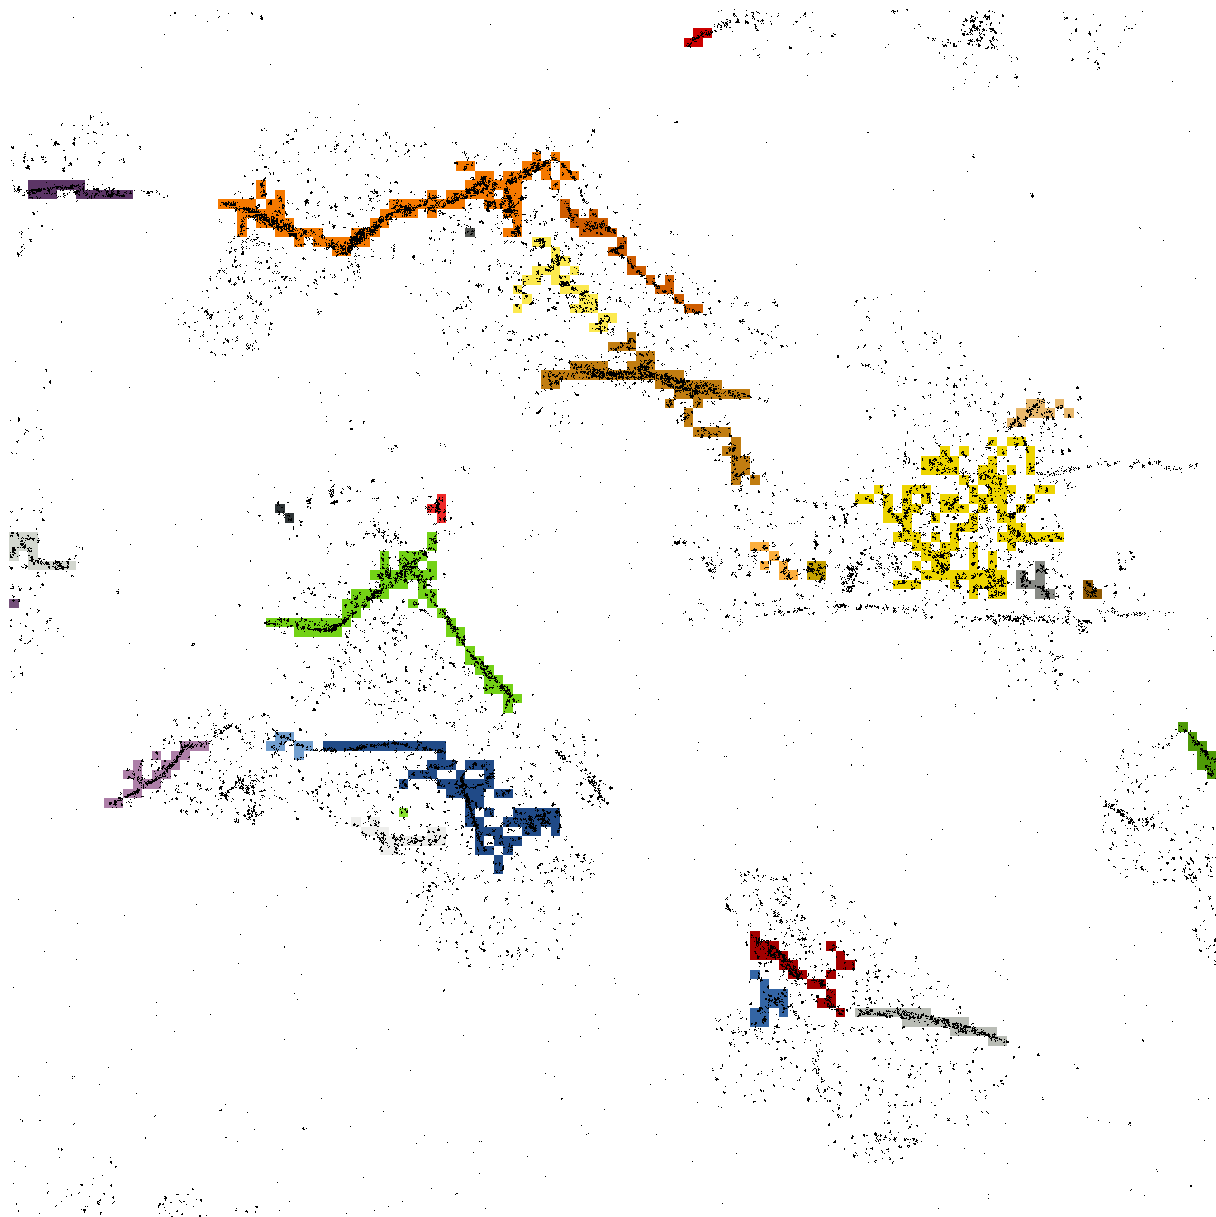
\includegraphics[width=\textwidth]{roundness-long.png}}
		\caption{}\label{fig:roundness-long.png}
	\end{subfigure}%
	\quad
	\begin{subfigure}[b]{4.2cm}
		\fbox{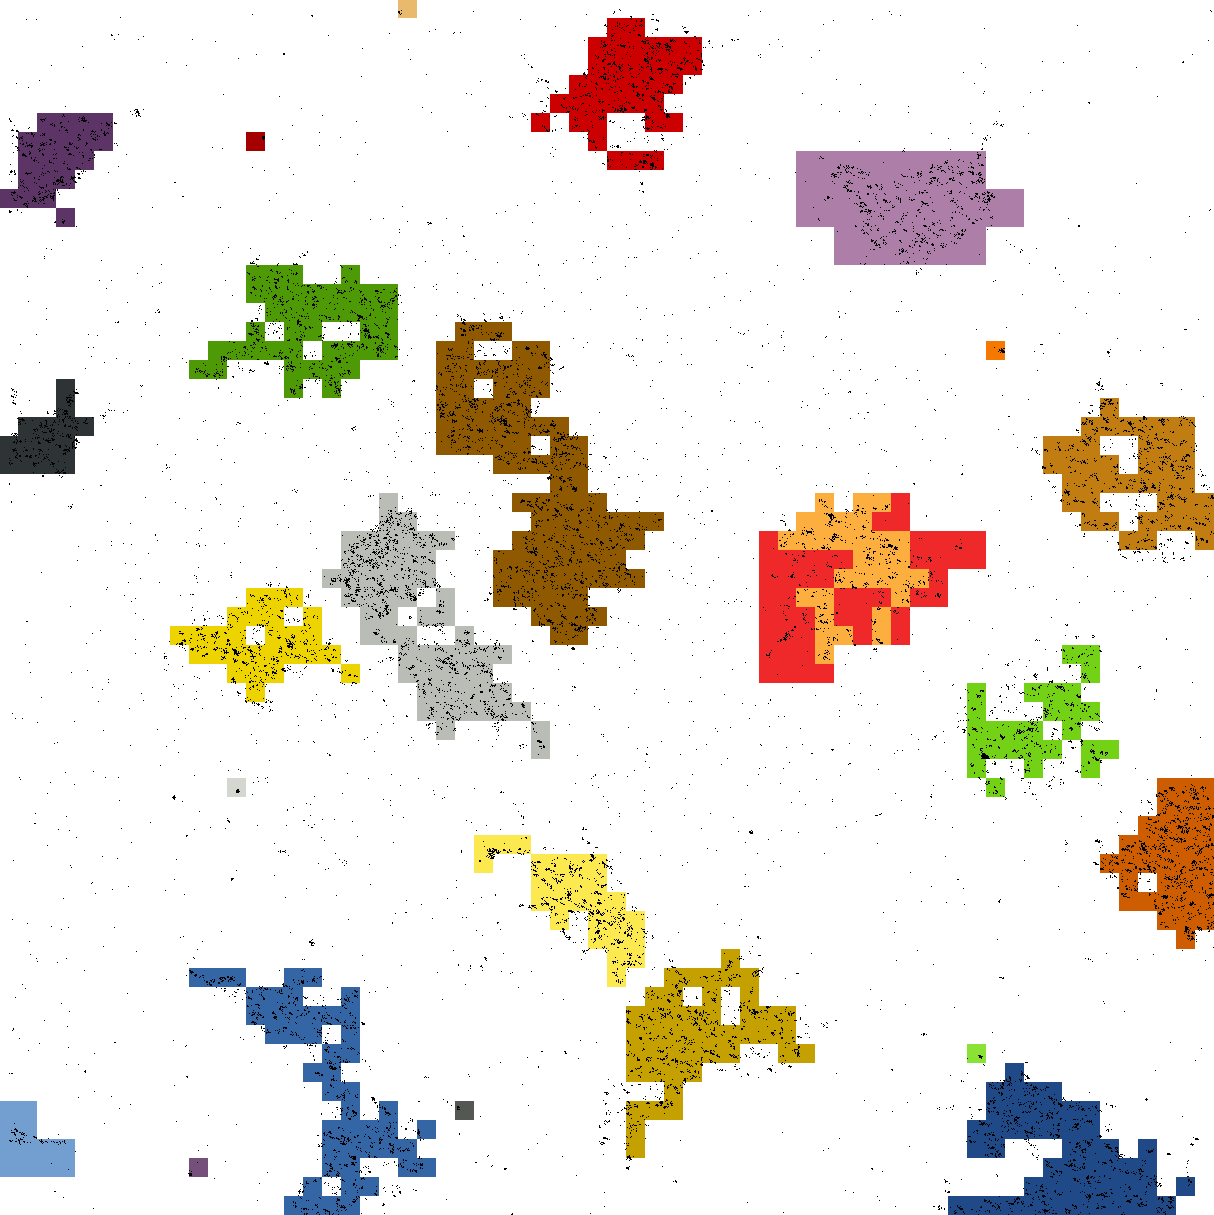
\includegraphics[width=\textwidth]{roundness-round.png}}
		\caption{}\label{fig:roundness-round.png}
	\end{subfigure}

	\caption[A comparison of roundness values.]{The general shape of the
		clusters found can be described using the roundness measure. A value
		closer to 0 means longer and thinner clusters, whereas values closer to
		1 mean clusters that are more circular.}\label{fig:roundness}
\end{figure}

\subsection{Point Analysis}
\label{sub:point_analysis}

Here, the points contained in the nodes of quadtree that were considered part
of the cluster are considered; the nodes are only used to select the correct
points.

\subsubsection{Cluster Perimeter}
\label{ssub:cluster_perimeter_point}

\subsubsection*{Convex Hull Algorithm}
\label{ssub:Convex Hull Algorithm}

There are a number of algorithms that atempt to find the bounding polygon of a
set of points. Ignoring any holes in the cluster, the perimeter of this bouding
polygon is equivalent to the perimeter of the cluster.

The simplest method of finding this bounding polygon is using the \emph{convex
hull} method\cite{barber1996quickhull}. In principle, this involves starting
with a circle far larger than the points it encloses, which is reduced in size,
without letting any point leave the shape, until only stright lines exist
between external points. The final shape can be pictured by imaginging each of
the points as being represented by a nail in a piece of wood. The convex hull
algorithm then calculates the shape that would be produced if an elastic band
were streched around these nails.

The major disadvantage of this algorithm is that, as the name suggest, the
final shape consists only of convex angles, meaning that the actual shape of
the perimeter of the points may be lost, as shown in
Figure~\ref{fig:convex-hull}.

\begin{figure}[tbhp]
	\centering
	\includegraphics[width=5cm]{convex-hull.pdf}

	\caption[Convex versus concave hull algorithms.]{Convex versus concave hull
		algorithms. The red line shows the convex hul found for this set of
		points, which misses much of the detail and will report the area as
		being significantly above its actual value. The blue line is the
		concave hull found.}\label{fig:convex-hull}
\end{figure}

\subsubsection*{Concave Hull Algorithm}
\label{ssub:Concave Hull Algorithm}

An alternative to the convex hull algorithm is the slightly more complex
\emph{concave} hull algorithm\cite{moreira2007concave}. Instead of simply
finding the outermost shape that will enclose all of the points, the concave
hull algorithm finds that shape that fits the outer boundary of the points more
closely. The steps involved are listed below.

\begin{enumerate}
	\item The algorithm looks at the distance to each of the nearest $n$
		points, where $n$ is specified beforehand.
	\item From these possibilities, it chooses the closest to be added to the
		``hull''.
	\item The new line segment that would be added by joining the existing hull
		to the new point is examined to ensure that it does not cross the
		existing hull at all.
	\item If it does cross, this point is removed as a possibility of being a
		part of the hull and the next nearest point is checked.
	\item When the initial starting point is reached again, the algorithm will
		have generated a closed loop joining a number of points togther.
	\item This closed loop is checked to ensure that all points lie either on
		the hull or are enclosed within it.
	\item If there are any points that fall outside the hull, the results are
		abandoned and the algorithm is re-run with the number of neighbours to
		check, $n$, incremented by one.
	\item When a hull is found that encloses all points, the algorithm
		terminates.
\end{enumerate}

\cite{lee2002polygonization}

\cite{estivill2000autoclust}

\cite{xia2006border}

% TODO mention delaunay triangulation
\cite{lee1980two}

\subsubsection{Cluster Area}
\label{ssub:cluster_area_point}

Once the perimeter hull of the cluster of points has been identified, it is
simple to calculate the area enclosed by that cluster from the hull. Since the
hull consists only of straight lines connecting single points, the area can be
calculated by splitting the polygon into regular triangles, and finding each of
their areas individually. The area of the whole cluster is then given by the
sum of these areas. An algorithm for calculating the area of the irregular
polygon produced with this method is shown in Listing~\ref{lst:polygon-area}.

\begin{center}
\begin{minipage}{\textwidth}
	\begin{lstlisting}[caption={[Code to find the area of an irregular
	polygon.]Code to find the area of an irregular polygon.  Adapted
	from~\cite{finley2006poly}}, label=lst:polygon-area] public
	|polygonArea(points, numPoints)| {

		area = 0;
		j = numPoints - 1;

		/* Sum the area contained between each pair of points and the y-axis on the right hand side of the shape and subtract the area between pairs of points and the y-axis on the left hand side. */
		for (i=0; i < numpoints; i++) {
			area += (points[j].getX() + points.[i].getX()) *
		        	(points[j].getY() - points.[i].getY());
			j = i;
		}
		return area/2;
	}
\end{lstlisting}
\end{minipage}
\end{center}


% Created:  Wed 13 Aug 2014 04:56 PM
% Author:   Josh Wainwright
% Filename: evaluation.tex

\part{Evaluation}
\label{prt:evaluation}

% Created:  Mon 01 Sep 2014 01:03 PM
% Author:   Josh Wainwright
% Filename: testing.tex

\section{Testing}
\label{sec:testing}

Since the absolute definition of the clusters that the plugin looks for are
somewhat subjective, testing the algorithm for correctness is difficult. The
individual functions and smaller components of the algorithms are tested using
the unit testing framework JUnit\cite{tahchiev2010junit}, and the overall
effectiveness of the clustering algorithms is validated with generated data
files and acceptance testing.

\subsection{Generated Test Files}
\label{sub:generated_test_files}

To try to test the algorithm and get some more quantitative results, it was
performed on a number of simulated test files. These data sets, shown in
Figure~\ref{fig:cam-tests} were produced by \citet{karypis1999chameleon} for
testing their Cameleon clustering algorithm. The algorithm was found to
identify 4 clusters in image (a) and a single cluster image (b), but performed
poorly in the final two.

\begin{figure}[tbh]
	\centering
	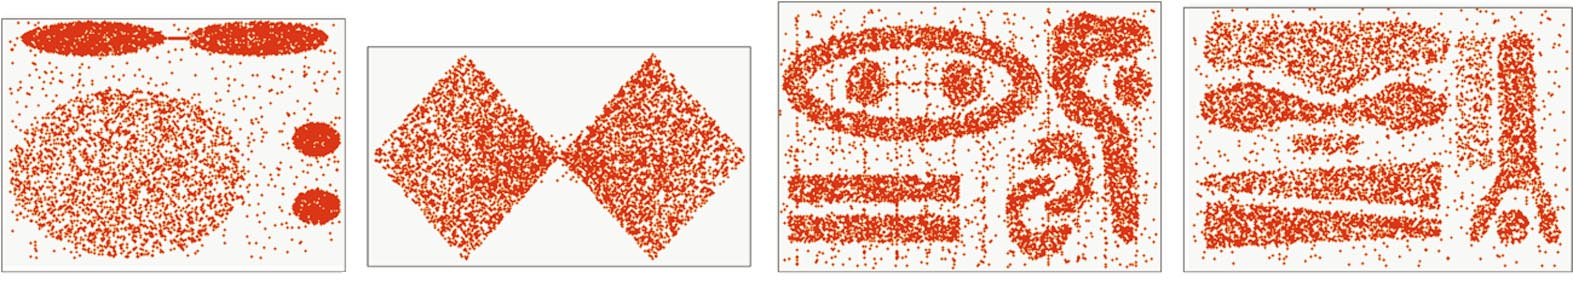
\includegraphics[width=0.9\linewidth]{cam-tests.png}
	\caption[Manually generated data sets for testing]{Manually generated data
		sets for testing. The images (a), (b), (c) and (d) above are used to
		test the algorithm for this project and for a number of other studies
		in clustering.}\label{fig:cam-tests}
\end{figure}

These particular datasets have been used to test a number of clustering
algorithms and so they provide a helpful benchmark with which these algorithms
can be compared. It is unfortunate that this algorithm fails to cope with the
complex structures that are present in the second two images, but shows that it
is more specifically taylored than the more general algorithms that use these
as tests. The clusters that the algorithm failed to identify lie too close
together meaning that the propagation step is able to cross from one cluster to
another.

The same effect is seen in images (a) and (b) where there is a link between
what would, otherwise, be separate clusters. This means the algorithm reports
these as a single object.

Another testing data set was created, similar to the final two images above,
but with more spacing to see how the algorithm would cope. An image of this set
is shown in Figure~\ref{fig:testing-image2a}.

\begin{figure}[tbh]
	\centering
	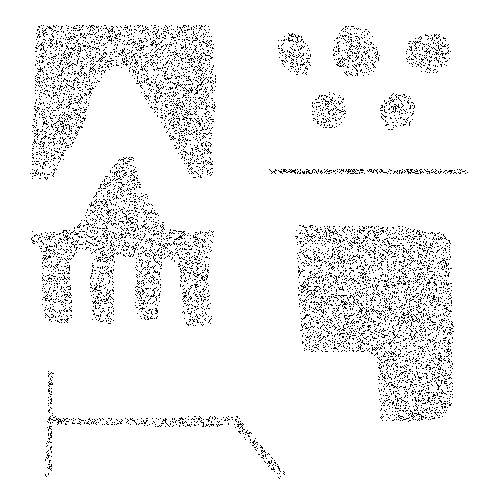
\includegraphics[width=0.5\linewidth]{testing-image2a.png}
	\caption[Custom generated data set for testing clustering
		algorithm.]{Custom generated data set for testing clustering
		algorithm. This data set is similar to that shown above, but
		has more space between clusters. The number of points in this
		% TODO Number of points in dataset.
		data set is .} \label{fig:testing-image2a}
\end{figure}

The results were better with this data set since the propagation step of the
algorithm was halted by the clear space between the clusters. When there is no
noise at all in the data, all of the clusters are located. The amount of noise
can be increased by simply adding random data points which are distributed
evenly across the image space. This is done progressively, adding TODO points
at a time. The clustering algorithm stops finding the clusters properly when
the number of noise points added is TODO. This represents when the noise to
signal ratio is TODO.

\subsection{Volunteer Validation}
\label{sub:volunteer_validation}

The first stage of acceptance testing took the form of a sample set of data
that was plotted onto an image using the discrete grid method. This data was
then presented to a number of volunteers who were asked to count the number of
clusters they could identify and then highlight the clusters that they were
able to observe in order of precedence, most defined through to least defined.

Once the volunteer had identified the clusters, the algorithm was performed on
the same set of data and the results compared to the predicted results.
Finally, when the algorithm identified clusters that the volunteers had not,
they were asked to identify which of these they did not consider to be valid
clusters and which were valid clusters that they had missed. The number of
false positive clusters identified by the quadtree algorithm was found, by this
method, to be low.

When using the settings described in Section~\ref{sub:option_sliders}, 100\% of
the clusters identified by the volunteers were able to be located by the
algorithm. Of the clusters that the algorithm found but the volunteers did not,
around 60\% were considered to be valid by the volunteers. These results
suggest that the algorithm is performing well at being able to identify
clusters, but requires some intervention to get the best results (see
Section~\ref{sec:possible_improvements}) and that, in general, the algorithm
does not produce that many false positive results.

\subsection{Researcher Validation}
\label{sub:researcher_validation}

The final stage of acceptance testing was performed to confirm the type of
clusters identified conformed with the actual objects that are being imaged.
This was performed by two researchers working in the medical imaging field who
produced the sample data used in this project.
% TODO

% Created:  Wed 13 Aug 2014 04:53 PM
% Author:   Josh Wainwright
% Filename: requirements.tex

\newgeometry{onecolumn}
\section{Requirements}
\label{sec:requirements}

% TODO Requirements intro
% TODO include explanation of MoSCoW

\subsection{Functional Requirements}
\label{sub:functional_requirements}

% TODO Functional Requirements

The plugin will allow the user to:

% \tabulinesep=1.2mm
% \newcounter{rowcount}
% \setcounter{rowcount}{-1}
% % TODO Don't have counter on header
% \begin{tabu}{@{\stepcounter{rowcount}\makebox[2em][r]{\therowcount.}\hspace*{\tabcolsep}}X c}
% 	\toprule
% 	Requirement & MoSCoW \\
% 	\midrule
% 	Select a data file to process.
% 	& M \\
% 	Select the appropriate column separator for the file.
% 	& C \\
% 	Select which coloumn the x- and y-coordinates appear in.
% 	& C \\
% 	Adjust parameters relating to the process of analysing the data file.
% 	& S \\
% 	Create an image of the points from the file using naitve ImageJ
% 	functionality.
% 	& S \\
% 	Perform a clustering algorithm on the data in the chosen file.
% 	& M \\
% 	Create an image of the clusters found using native ImageJ functionality.
% 	& M \\
% 	Generate perimeter information for each of the clusters found.
% 	& S \\
% 	Generate area information for each of the clusters found.
% 	& S \\
% 	Display a results table showing summary of information about each of the
% 	clusters found.
% 	& S \\
% 	Limit the clusters drawn to the image based on the size of the cluster.
% 	& C \\
% 	Limit the clusters included in the results table based on the size of the
% 	cluster.
% 	& C \\
% 	Export cluster information by selecing appropriate cluster from the results
% 	table.
% 	& W \\
% 	Export data points contained in cluster by selecing appropriate cluster
% 	from the results table.
% 	& W \\
% 	\bottomrule
% \end{tabu}

\begin{enumerate}
	\item Select data
		\begin{enumerate}
			\item Select a data file to process.
			\item Select the appropriate column separator for the file.
			\item Select which coloumn the x- and y-coordinates appear in.
			\item Adjust parameters relating to the process of analysing the
				data file.
		\end{enumerate}
	\item Create images
		\begin{enumerate}
			\item Create an image of the points from the selected file using
				naitve ImageJ functionality.
			\item Create an image of the clusters found using native ImageJ
				functionality.
		\end{enumerate}
	\item Perform a clustering algorithm on the data in the chosen file.
	\item Generate cluster information
		\begin{enumerate}
			\item Generate perimeter information for each of the clusters found.
			\item Generate area information for each of the clusters found.
			\item Display a results table showing summary of information about each of the clusters found.
			\item Limit the clusters drawn to the image based on the size of the cluster.
			\item Limit the clusters included in the results table based on the size of the cluster.
		\end{enumerate}
	\item Export data found by the algorithm.
		\begin{enumerate}
			\item Export cluster information by selecing appropriate cluster from the results table.
			\item Export data points contained in cluster by selecing appropriate cluster from the results table.
		\end{enumerate}
\end{enumerate}

\subsection{Non-Functional Requirements}
\label{sub:non_functional_requirements}

% TODO Non-Functional Requirements

The plugin will:

\begin{enumerate}
	\item Handle input data files of upto 3 million data points.
		% TODO test this
\end{enumerate}

\restoregeometry

% Created:  Thu 28 Aug 2014 10:09 AM
% Author:   Josh Wainwright
% Filename: development.tex

\section{Development Evaluation}
\label{sec:development_evaluation}

The development process of this project followed an agile methodology. There
was a distinction in steps between the initial design of the data structures
and algorithms and the development of the program and the plugin for ImageJ.
There were stages of development of the algorithms and the plugin which were
revisited a number of times during the development. At each stage, the plugin
was tested and any bugs fixed before new features or the next algorithms were
added.

\subsection{Future Work}
\label{sub:future_work}

% TODO future work

\subsection{Development Process}
\label{sub:development_process}

The estimated schedule that were proposed prior to the start of development
are listed in Table~\ref{tab:schedule}. This was followed reasonably closely
throughout the project, though some deviations were encountered when the
development of algorithms took longer than was expected. In particular, issues
when designing the modified Gray code quadtree ordering slowed development
significantly. See Section~\ref{ssub:Chosen Ordering} for the reasons. To
account for these changes, other stages were allocated slightly less time than
is recorded here.

\begin{table}
\begin{tabu} to \linewidth{c X l}
	\toprule
	Stage & Tasks & Date \\
	\midrule
	1  & Research existing methods of cluster analysis and identify short comings.         & 20th June 2014 \\
	2  & Build implementation of Uniform Discrete Cell method.                             & 27th June 2014 \\
	3  & Build implementation of Quadtree method.                                          & 11th July 2014 \\
	4  & Test and compare previous algorithms. Perform timing and resource usage analysis. & 18th July 2014 \\
	5  & Build first iteration ImageJ plugin using chosen method.                          & 25th July 2014 \\
	6  & Using chosen method, implement cluster analysis algorithms.                       & 1th August 2014 \\
	7  & Add cluster analysis to ImageJ plugin.                                            & 8th August 2014 \\
	8  & Performance and ease of use testing of plugin.                                    & 15th August 2014 \\
	9  & Write-up of background research and current implementations investigation         & 18th July 2014 \\
	10 & Write-up of data structure algorithms.                                            & 1st August 2014 \\
	11 & Write-up of cluster analysis algorithms.                                          & 22nd August 2014 \\
	12 & Final write-up of processes, improvements and end results of project.             & 29th August 2014 \\
	\bottomrule
\end{tabu}
\caption{An initially proposed schedule for the development process. The dates
	were not followed exactly, but the tasks were performed in this
	order.}\label{tab:schedule}
\end{table}

% Created:  Thu 24 Jul 2014 04:40 PM
% @author Josh Wainwright
% filename: improvements.tex

\section{Possible Improvements}
\label{sec:possible_improvements}

Though the primary  aims of this project were fulfilled, there are a few areas
that could be improved, or features that could be added that would improve the
plugin and make it easier to use. These features were not developed during the
course of this project because the core functionality was more important and
time constraints prevented them from being added after the existing features
were complete.

\begin{description}

	\item[Alternative algorithms] \hfill

		The algorithm that was developed for this project performs well under a
		range of different conditions. This was tested through the use of
		exemplar data sets and data sets constructed for use in testing to
		simulate different conditions. However, there may be some situations
		that were not tested for which it might not perform well. To avoid
		this, a number of alternative algorithms could be included so that, if
		the default algorithm fails, the user could switch to a different
		approach which might handle the data better.

		One or more of the existing algorithms discussed in
		Part~\ref{prt:existing_cluster_analysis_algorithms} could be
		implemented as alternatives which could then be selected from the main
		user interface if the quadtree based method failed.

	\item[Better starting location selection] \hfill

		The logic in the current implementation that selects new starting
		locations where clusters are propagated from is reasonably simple and
		so can fail to determine the best next location. This would be improved
		by a method that considered more than simply the quadtree structure,
		such as the placement of existing clusters and the depth of node
		surrounding the possible starting location.

	\item[Better algorithm halting] \hfill

		Similarly to above, the logic that stops the algorithm looking for
		more starting locations once a cluster has finished being propagated
		are not always sufficient. For example, in a data set with few
		clusters, zero to six, the algorithm will continue to look for more and
		so might identify the background noise as a cluster that spans most of
		the image.

	\item[Calculation of optimum settings] \hfill

		Since the particular settings that are required vary a lot between
		different data sets, the user must often alter the settings before any
		useful results are found. To automate this process would require some
		significant changes to the algorithm so that it did not take a
		prohibitive amount of time to produce results, but would make the
		plugin far easier to use.

\end{description}


% \clearpage
% \newgeometry{onecolumn,top=2in,left=1.5in,right=1.5in}
\onecolumn
% \thispagestyle{empty}
\nocite{*}
\bibliographystyle{apalike}
\bibliography{references}

\clearpage
% Created:  Sun 15 Jun 2014 04:27 pm
% Modified: Mon 23 Jun 2014 01:07 PM

\appendix
\addcontentsline{toc}{part}{Appendices}

% Created:  Mon 23 Jun 2014 04:06 PM
% @author Josh Wainwright
% File name : file-columns.tex

\section{Data File Structure}
\label{app:data_file_structure}

The data files that are produced from the initial analysis of the images have a
standard format.

\begin{enumerate}
	\item Tab separated fields.
	\item Single header line with names of fields.
	\item One or more item of data, separated by newlines.
\end{enumerate}

The columns that represent fields in the file are as follows.

\begin{center}
	\begin{tabu}{p{1.1cm} X c}
		\toprule
		Header & Meaning & Used? \\
		\midrule
		\texttt{Channel Name} & Wavelength channel that was used to capture data.
			First value, $I$, is the incident wavelength of the light used to
			excite the dye and the second, $E$, is the wavelength emitted that
			was imaged. & no \\
		\texttt{X} & x-coordinate of the point & no \\
		\texttt{Y} & y-coordinate of the point & no \\
		\texttt{Xc} & centered, normalised x-coordinate of point & yes \\
		\texttt{Yc} & centered, normalised y-coordinate of point & yes \\
		\texttt{Height} & the height of the fitted Gaussian peak used to
			extract the point from the original image & not yet \\
		\texttt{Area} & area of the point & not yet \\
		\texttt{Width} & full width half maximum of the point & not yet \\
		\texttt{Phi}          &  & no \\
		\texttt{Ax}           &  & no \\
		\texttt{BG}           &  & no \\
		\texttt{I}            &  & no \\
		\texttt{Frame}        &  & no \\
		\texttt{Length}       &  & no \\
		\texttt{Valid}        &  & no \\
		\texttt{Z}            &  & no \\
		\texttt{Zc}           &  & no \\
		\texttt{Photons}      &  & no \\
		\texttt{Lateral Localisation Accuracy}     &  & no \\
		\texttt{Xw}           &  & no \\
		\texttt{Yw}           &  & no \\
		\texttt{Xwc}          &  & no \\
		\texttt{Ywc}          &  & no \\
		\bottomrule
	\end{tabu}
\end{center}



\restoregeometry

\end{document}
